\documentclass[12pt,          % font size: 11pt or 12pt
               ms,           % degree:    ms or phd
               doublespacing % spacing: onehalfspacing or doublespacing
               ]{ncsuthesis}

%%----------------------------------------------------------------------------%%
%%------------------------------ Import Packages -----------------------------%%
%%----------------------------------------------------------------------------%%

\usepackage{booktabs}  % professionally typeset tables
\usepackage{amsmath}%,amssymb,amsfonts}
\usepackage{textcomp}  % better copyright sign, among other things
%\usepackage{xcolor}
\usepackage{lipsum}    % filler text
\usepackage{subfig}    % composite figures

%%ORTIZ PACKAGES


%%%%%%%%%%%%%%%%%%%%%%%%%%%%%%%%%%%%%%%%%%
%%%%%%%%%%% Old bibliography commands
%%%%%%%%%%%%%%%%%%%%%%%%%%%%%%%%%%%%%%%%%%5
%\usepackage[super,sort&compress,comma,square,authoryear]{natbib} %\cite command %Added by Ortiz

%use the following line with plainnat
%\usepackage[super,sort&compress,comma,square,numbers]{natbib} %\cite command %Added by Ortiz
%\usepackage{natbib}

%\usepackage[style=alphabetic,natbib=true,backend=bibtex
%sorting=nyt,firstinits=true,isbn=false,doi=false,url=false]{biblatex} %couldn't get backend=biber to work

%\usepackage{filecontents}

%\bibliography{Ortiz-thesis2}
%\bibliographystyle{plain}


%%%%%%%%%%%%%%%%%%%%%%%%%%%%%%%%%%%%%%%%%%
%%%%%%%%%%% Hack for alphanumeric bibliography
%%%%%%%%%%%%%%%%%%%%%%%%%%%%%%%%%%%%%%%%%%5
\RequirePackage[
			style=alphabetic,%numeric-comp,%authoryear-comp,%
			sorting=nyt,%ynt					
			hyperref=true, %	
			firstinits=true,%
			backend=bibtex,
			natbib=true,
			url=false,
			isbn=false,
			maxnames=2, %for et al to be used
			maxalphanames=1, %to avoid printing a + for every et al in the abbreviation
			doi=false]{biblatex}		
			

%needed to do et al after two names
%http://tex.stackexchange.com/questions/44048/use-et-al-in-biblatex-custom-style
\renewcommand*{\finalnamedelim}{\addspace\&\space}

%Simplify abbreviation (the default uses either one or two authors and it indicates et al with a +)
%The following five lines make it so that only the first author is used in the abbreviation
%http://tex.stackexchange.com/questions/27956/label-only-from-first-author
\renewcommand*{\labelalphaothers}{}
    \renewcommand*{\intitlepunct}{}
    \DefineBibliographyStrings{german}{in={}}
    \DefineBibliographyStrings{english}{in={}}
    \DeclareNameAlias{sortname}{last-first}
    \DeclareNameAlias{default}{last-first}
	
%\AtEveryCitekey{\ifciteseen{}{\defcounter{maxnames}{99}}} %authoryear			
\DeclareFieldFormat[article,periodical]{volume}{\mkbibbold{#1}}
\makeatletter

\newrobustcmd*{\parentexttrack}[1]{%
  \begingroup
  \blx@blxinit
  \blx@setsfcodes
  \blx@bibopenparen#1\blx@bibcloseparen
  \endgroup}

\AtEveryCite{%
  \let\parentext=\parentexttrack%
  \let\bibopenparen=\bibopenbracket%
  \let\bibcloseparen=\bibclosebracket}

\makeatother
\renewcommand{\cite}[1]{\parencite{#1}}


\renewbibmacro{in:}{%
  \ifentrytype{article}{}{%
  \printtext{\bibstring{in}\intitlepunct}}}
  
\AtEveryBibitem{\clearfield{month}}

\AtEveryBibitem{\clearfield{language}}
%%%%%%%%%%%%%%%%%%%%%%%%%%%%%%%%%%%%%%%%%%%%%

%\addbibresource{Ortiz-thesis2.bib}
%\addbibresource{Ortiz-thesisURL.bib}
\addbibresource{YourName-thesis.bib}

 \defbibheading{myheading}[BIBLIOGRAPHY]{
 \chapter*{#1}
 %\centerline{\bf{#1}}
 \markboth{#1}{#1}}

%\usepackage{amsmath,amssymb,amsfonts} %amssymb and amsfonts cannot be used in conjunction with mdput
%\usepackage{graphicx,subfig}% Include figure files
\usepackage{dcolumn}% Align table columns on decimal point
\usepackage{bm}% bold math
%\usepackage{hyperref}% add hypertext capabilities
%\usepackage{hypernat}% make hyperref and natbib work together
\usepackage{cancel}
\usepackage{verbatim}% multiline commenting
\usepackage{ifthen}
\usepackage{url}
\usepackage{sectsty}
\usepackage{balance} 
%\usepackage{caption}
\usepackage{graphicx} %eps figures can be used instead
\usepackage{lastpage}
\usepackage[format=plain,justification=RaggedRight,singlelinecheck=false,font=small,labelfont=sf,labelsep=space]{caption} 
\usepackage{fancyhdr}
\pagestyle{fancy}

%http://tex.stackexchange.com/questions/100817/error-when-using-bc-from-abbrevs-in-caption
%Getting BC
\usepackage{abbrevs}
\usepackage{etoolbox}
\robustify{\DateMark} % after having loaded abbrevs

\usepackage{units} %Needed to solve bug from citation Hydrodynamics in 21/2 dimensions
%see http://www.latex-community.org/viewtopic.php?f=5&t=989

\usepackage[sharp]{easylist} %used for brainstorming purposes 
%\usepackage{mathabx} % used for \Asterisk for convolution %conflicts with \widering

%compile on single pass
%\usepackage[backend=biber,...]{biblatex}


%%%%%%%%%%%%
%%% Hack to make chapters start on odd pages
% http://tex.stackexchange.com/questions/73591/how-to-have-a-blank-even-page-before-every-chapter
%%%%%%%%%%%%
%\newcommand{\ensureoddstart}{\checkoddpage\ifoddpage\else\newpage\mbox{}\fi}
%\newcommand{\ensureoddstart}{}


%%%Fancy tables
%http://tex.stackexchange.com/questions/94032/fancy-tables-in-latex
\usepackage[table]{xcolor}
\usepackage{array,booktabs}
\usepackage{colortbl}
\newcolumntype{L}{@{}>{\kern\tabcolsep}l<{\kern\tabcolsep}}



%%%%%%%%%%
%%%%% Hack to allow more levels in outline
%%%%%%%%%%
%\setcounter{secnumdepth}{5}
%\setcounter{tocdepth}{5} %may violate ETD
%Usage http://pleasemakeanote.blogspot.com/2010/06/how-to-activate-subsubsubsection-in.html
%\section{} % level 1
%\subsection{} % level 2
%\subsubsection{} % level 3
%\paragraph{} % level 4 - equivalent to subsubsubsection
%\subparagraph{} % level 5

%http://tex.stackexchange.com/questions/60209/how-to-add-an-extra-level-of-sections-with-headings-below-subsubsection
\usepackage{titlesec}

\setcounter{secnumdepth}{4}

\titleformat{\paragraph}
{\normalfont\normalsize\bfseries}{\theparagraph}{1em}{}
\titlespacing*{\paragraph}
{0pt}{3.25ex plus 1ex minus .2ex}{1.5ex plus .2ex}


%%%%%%%%%%%%%%%%%%%%%%%%%%
%%%% Hack for containing figures within sections
%%%%%%%%%%%%%%%%%%%%%%%%%%%%
%http://ctan.org/pkg/placeins
\usepackage{placeins}
%De�fines a \FloatBar�rier com�mand, be�yond which floats may not pass; use�ful, for ex�am�ple, to en�sure all floats for a sec�tion ap�pear be�fore the next \sec�tion com�mand.

%%%Hack for centering all figures
%\makeatletter
%\g@addto@macro\@floatboxreset\centering
%\makeatother

%%----------------------------------------------------------------------------%%
%%---------------------------- Formatting Options ----------------------------%%
%%----------------------------------------------------------------------------%%
%%

%% -------------------------------------------------------------------------- %%
%% Disposition format -- any titles, headings, section titles
%%  These formatting commands affect all headings, titles, headings,
%%  so sizing commands should not be used here.
%%  Formatting options to consider are
%%     +  \sffamily - sans serif fonts.  Dispositions are often typeset in
%%                    sans serif, so this is a good option. 
%%     +  \rmfamily - serif fonts
%%     +  \bfseries - bold face
%\dispositionformat{\sffamily\bfseries}   % bold and sans serif
\dispositionformat{\rmfamily}            % bold and serif

%% -------------------------------------------------------------------------- %%
%% Formatting for centered headings - Abstract, Dedication, etc. headings
%%  This is where one might put a sizing command.
%%  \MakeUppercase can be used to typeset all headings in uppercase.
\headingformat{\large\MakeUppercase}   % All letters uppercase
%\headingformat{\large}                % Not all uppercase
%\headingformat{\Large\scshape}        % Small Caps, used with serif fonts.

%% Typographers recommend using a normal inter-word space after
%% sentences. TeX's default is to add an wider space, but \frenchspacing
%% gives a normal spacing. Comment out the following line if you prefer
%% wider spaces between sentences.
\frenchspacing


%% -------------------------------------------------------------------------- %%
%%  Optional packages
%%    A number of compatible packages to improve the look and feel of
%%    your document are available in the file optional.tex 
%%    (For example, hyperlinks, fancy chapter headings, and fonts)
%% To use these options, uncomment the next line and see optional.tex
%%  Optional Packages to consider.   These packages are compatible with
%%    ncsuthesis.  

%% -------------------------------------------------------------------------- %%
%% Fancy chapter headings
%%  available options: Sonny, Lenny, Glenn, Conny, Rejne, Bjarne
%\usepackage[Sonny]{fncychap}
\usepackage[Rejne]{fncychap}

%%----------------------------------------------------------------------------%%
%% Hyperref package creates PDF metadata and hyperlinks in Table of Contents
%%  and citations.  Based on feedback from the NCSU thesis editor, 
%%  the links are not visually distinct from normal text (i.e. no change
%%  in color or extra boxes).
\usepackage[
  pdfauthor={Carlos Pompeyo Ortiz},
  pdftitle={Rigidity of Microsphere Heaps},
  pdfcreator={pdftex},
  pdfsubject={NC State ETD Thesis},
  pdfkeywords={microfluidics, hard sphere, jamming, suspension, rigidity, friction, microscopy},
  colorlinks=true,
  linkcolor=black,
  citecolor=black,
  filecolor=black,
  urlcolor=black,
]{hyperref}

%%----------------------------------------------------------------------------%%
%% table of contents bold fix
\usepackage{tocloft}
\renewcommand\cftchapfont{\mdseries}
\renewcommand\cftchappagefont{\mdseries}


%% -------------------------------------------------------------------------- %%
%% Microtype - If you use pdfTeX to compile your thesis, you can use
%%              the microtype package to access advanced typographic
%%              features.  By default, using the microtype package enables
%%              character protrusion (placing glyphs a hair past the right 
%%              margin to make a visually straighter edge)
%%              and font expansion (adjusting font width slightly to get 
%%              more favorable justification).
%%              Using microtype should decrease the number of lines
%%              ending in hyphens.
\usepackage{microtype}


%%----------------------------------------------------------------------------%%
%% Fonts 

%% ETD guidelines don't specify the font.  You can enable the fonts
%%  by uncommenting the appropriate lines.  Using the default Computer 
%%  Modern fonts is *not* required.  A few common choices are below.
%%  See http://www.tug.dk/FontCatalogue/ for more options.

%% Serif Fonts -------------------------------------------------
%%  The four serif fonts listed here (Utopia, Palatino, Kerkis,
%%  and Times) all have math support.


%% Utopia
\usepackage[T1]{fontenc}
\usepackage[adobe-utopia]{mathdesign}

%% Palatino
%\usepackage[T1]{fontenc}
%\usepackage[sc]{mathpazo}
%\linespread{1.05}

%% Kerkis
%\usepackage[T1]{fontenc}
%\usepackage{kmath,kerkis}

%% Times
%\usepackage[T1]{fontenc}
%\usepackage{mathptmx}


%% Sans serif fonts -------------------------

%\usepackage[scaled]{helvet}  % Helvetica
%\usepackage[scaled]{berasans} % Bera Sans

%solve bug from fancyhdr in optional
%http://nw360.blogspot.com/2006/11/latex-headheight-is-too-small.html
\setlength{\headheight}{14pt}

%%----------------------------------------------------------------------------%%
%%---------------------------- Content Options -------------------------------%%
%%----------------------------------------------------------------------------%%
%% Size of committee: 3, 4, 5, or 6 -- this number includes the chair
\committeesize{3}

%% Members of committee
%%  Each of the following member commands takes an optional argument
%%   to specify their role on the committee.
%%  For co-chairs, use the commands:
%%      \cochairI{Doug Dodd}
%%      \cochairII{Chris Cox}
%%
\chair{Dr. Yun Jing}
\memberI{Dr. Lawrence Silverberg}
\memberII{Dr. Marie Muller}


%% Student writing thesis, \student{First Middle}{Last}
\student{Sean Casey}{Maguire} % a full middle name
%\student{John M.}{Smith} % a middle initial

%% Degree program
\program{Mechanical Engineering}

%% Thesis Title
%%  Keep in mind, according to ETD guidelines:
%%    +  Capitalize first letter of important words.
%%    +  Use inverted pyramid shape if title spans more than one line.
%%
%%  Note: To break the title onto multiple lines, use \break instead of \\.
%\thesistitle{A North Carolina State University Sample \LaTeX{} Thesis \break 
%with a Title So Long it Needs a Line Break}
\thesistitle{Exploration of Cellulose Acetate Tow for Acoustic Control\break}

%% Degree year.  Necessary if your degree year doesn't equal the current year.
%\degreeyear{1995}


%%----------------------------------------------------------------------------%%
%%---------------------------- Personal Macros -------------------------------%%
%%----------------------------------------------------------------------------%%

%% A central location to add your favorite macros.

%% A few examples to get you started.
\newcommand{\uv}[1]{\ensuremath{\mathbf{\hat{#1}}}}
\newcommand{\bo}{\ensuremath{\mathbf{\Omega}}}
\newcommand{\eref}[1]{Eq.~\ref{#1}}
\newcommand{\fref}[1]{Fig.~\ref{#1}}
\newcommand{\tref}[1]{Table~\ref{#1}}
\newcommand{\del}{\nabla}
\renewcommand{\exp}[1]{e^{#1}}
\newcommand{\Conv}{\mathop{\scalebox{1.5}{\raisebox{-0.2ex}{$\ast$}}}}%


\usepackage{color}
%\newcommand{\NEW}[1]{\textcolor{blue}{#1}}
\newcommand{\NEW}[1]{#1}
\newcommand{\COMMENT}[1]{\textcolor{green}{#1}}


\newcommand{\NOTER}[1]{\textcolor{orange}{#1}}
\newcommand{\NOTEC}[1]{\textcolor{blue}{#1}}
\newcommand{\NOTEK}[1]{\textcolor{magenta}{#1}}

\newcommand{\mum}{\ensuremath{{\mu}\text{m}}}

%This makes it so that you can add short paths in your .tex by including the folders where you store your images in the search path
\graphicspath{{./Chapter-1/figs/}{./Chapter-2/figs/}{./Chapter-3/figs/}}%{./Chapter-4/figs/}{./Chapter-5/figs/}{./Chapter-6/figs/}}


%%---------------------------------------------------------------------------%%
\usepackage{calc}
%% Capital letter height
\newlength{\chaptercapitalheight}
\settoheight{\chaptercapitalheight}{D}
\newlength{\chapterfootskip}
\setlength{\chapterfootskip}{\chaptercapitalheight}
\addtolength{\chapterfootskip}{2\baselineskip}
\addtolength{\chapterfootskip}{0.5ex}  % A little extra space to ensure there are 2 full double spaced lines
%\def\chapterfootskipnum{\chapterfootskip}
\renewcommand{\listfigurename}{LIST OF FIGURES}
\renewcommand{\listtablename}{LIST OF TABLES}
\renewcommand{\bibname}{BIBLIOGRAPHY}

%\renewcommand{\cfttoctitlefont}{\centering\ncsu@headingformat}


%http://tex.stackexchange.com/questions/47184/height-of-figure-caption-textheight
\newlength\graphht
\newcommand\calculategraphicstargetheight[1]{%
     \setlength\graphht{\textheight 
                       -\parskip
                       -\abovecaptionskip -\belowcaptionskip
                       -(12pt * #1) % assuming baselineskip of 12pt in caption
                       -\chapterfootskip
                       }}

%\usepackage{titlesec}

%landscape support in fancyhdr from http://tex.stackexchange.com/questions/9071/how-to-translate-and-rotate-the-heading-of-landscaped-pages
\usepackage{pdflscape}
\usepackage{tikz}
\fancypagestyle{lscapedplain}{%
  \fancyhf{}
  \fancyfoot{%
    \tikz[remember picture,overlay]
      \node[outer sep=1cm,above,rotate=90] at (current page.east) {\thepage};}
\renewcommand{\headrulewidth}{0pt} 
\renewcommand{\footrulewidth}{0pt}
}
\usepackage{indentfirst}
\begin{document}
\pagestyle{plain}
%%---------------------------------------------------------------------------%%
\frontmatter
%% ------------------------------ Abstract ---------------------------------- %%
\begin{abstract}
The study of acoustic properties of porous materials has been of interest in many research publications in recent years. Noise pollution is considered to be a major health concern in both homes and places of employment. A means of solving this issue is the use of absorption materials to provide control over the acoustics in a given environment.  As is a trend in many industries, environmentally and biologically friendly materials have become a topic of growing interest. The objective of this research is to present an investigation of Cellulose Acetate Tow (CA) for use as an acoustic absorption material. Analysis of this material was performed via experimental data collected from a Br�el \& Kj�r Impedance/Transmission Loss Measurement Tube Type 4206A system to analyze the characteristic absorption coefficient $\alpha_c$ with respect to frequency $f$. The frequency range from $50$ Hz to $6300$ Hz was analyzed. Various form factors of CA have been tested. Experimental results are shown with respect to commercial acoustic absorption media of similar form factor. CA materials with high denier weight have shown similar performance to fiberglass, which is a current standardized material in the industry. Due to the complex nature of porous media absorption problems, the key poroelastic parameters needed for optimization are difficult to identify. As the experimental data reflects, Cellulose Acetate shows promise as an effective alternative to current materials.
\end{abstract}
%% ---------------------------- Copyright page ------------------------------ %%
%% Comment the next line if you don't want the copyright page included.
\makecopyrightpage
%% -------------------------------- Title page ------------------------------ %%
\maketitlepage
%% -------------------------------- Dedication ------------------------------ %%
\begin{dedication}
\centering{To my Mom, Dad, and Brother.}
\end{dedication}
%% -------------------------------- Biography ------------------------------- %%
\begin{biography}
Sean Casey Maguire was born in Cary, North Carolina on January 11$^\text{th}$, 1991. Sean attended North Carolina State University and received a Bachelor of Science degree in Aerospace Engineering in May 2013. During his undergraduate degree, Sean had the opportunity to travel to Hangzhou, China and Valencia, Spain. While abroad, Sean completed a minor in Spanish Language. His academic career continued at North Carolina State University where he is pursuing a Master of Science degree in Mechanical Engineering.\\
\indent Apart from his research in graduate school, Sean also helped design GUI applications for Mathworks. He works part-time as an Engineering Intern at Cree, Inc. in Durham, North Carolina. In his free time, Sean enjoys music, traveling to new places, basketball, and spending time with his friends.
\end{biography}
%% ----------------------------- Acknowledgements --------------------------- %%
\begin{acknowledgements}
I would like to thank first and foremost my advisor, Dr. Yun Jing for all his guidance and support in my research.\\
\indent I would also like to thank my lab mates in the Acoustics and Ultrasonics Laboratory for their support over the last year of research and classwork.\\
\indent I would like to thank my graduate committee, Dr. Lawrence Silverberg and Dr. Marie Muller for providing valuable input on my thesis and research.\\
\indent Last but not least, I would like to thank, Damon Billodeaux and the entire Eastman Chemical Company Innovation Center, and Aaron Kelley and Auralex Acoustics for their advice and assistance with experiments.
\end{acknowledgements}
\thesistableofcontents
\thesislistoftables
\thesislistoffigures
%%---------------------------------------------------------------------------%%
\mainmatter
\pagestyle{fancy}
\newgeometry{margin=1in,lmargin=1.25in,footskip=\chapterfootskip, includehead, includefoot}
\chapter{INTRODUCTION}
\label{chap-one}

\section*{Introduction}

This Chapter provides an introduction into sound propagation in porous materials.

\section{Motivation}

The study of acoustic properties of porous materials has been of interest in many research publications in recent years \cite{Horoshenkov2013}. Noise pollution is considered to be a major health concern in both homes and places of employment. It has been shown that exposure to large durations and magnitudes of sound results in permanent loss of hearing and damage to cells \cite{Bohne2007}. A means of solving this issue is the use of absorption materials to provide control over the acoustics in a given environment. Noise control solutions have a broad range of applications such as the industrial, automotive, architectural and medical fields. \cite{Beranek1969} \cite{Shoureshi1996} \cite{Horoshenkov2013}. In recent years, environmentally and biologically friendly materials have gained interest as a research subject. \cite{Ersoy2009} \cite{Wassilieff1996}. Currently, the sound absorption market is dominated with glass wool, foam and fibrous materials which prove to be the most valuable materials. However, many of these materials are not the best suited for close contact with humans. For example, fiberglass which is a common absorption material, has hazardous effects when ingested by an individual. For this reason, biologically friendly porous materials as alternatives to current solutions are of interest. An advantage to these materials is that they allow for sound damping in desirable, however previously unfeasible locations and applications such as dampening in the medical setting.

\section{Applications}

\subsection{Acoustics}
The ability to control the sound pressure levels in a room is desirable to engineers, architects and acousticians alike. Modern day architecture goes to great lengths to consider the level of noise pollution in a space. This ranges from industrial, automotive, musical, and education space applications. It also has a wide range of practical uses in daily life. \cite{Beranek1969} \cite{Shoureshi1996}.

In general, there exist various acoustic treatments which need to be considered when designing the acoustic space in a room. The treatments focus on absorption, reflection and diffusion \cite{Cox2004}. Figure \ref{fig:acoustictreaments} shows how each of these vary. The focus for noise controllability is the absorption treatment. The ability to control noise stems from 3 key principles. These are absorption, specular reflection and diffuse reflection as can be seen in Figure \ref{fig:noisecontrol}. Absorption is the key variable. 

% Acoustic Treatments
\begin{figure}[hbtp]
    \centering
    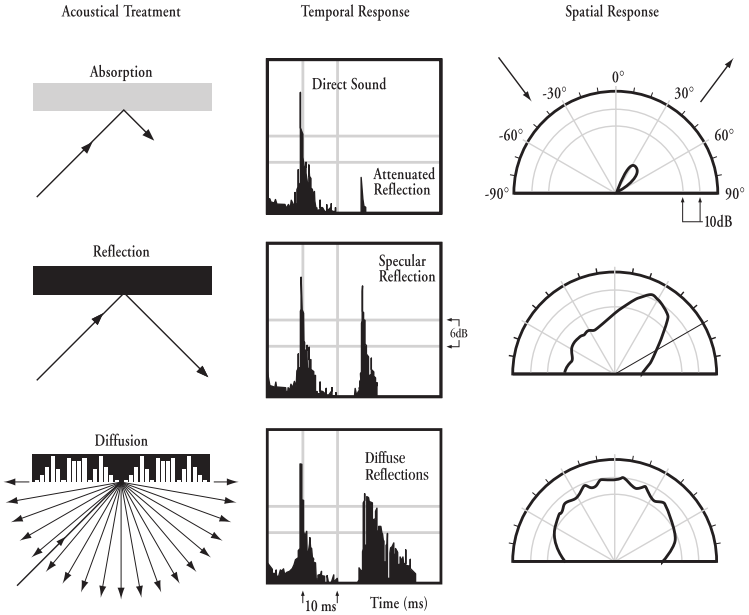
\includegraphics[width=1\textwidth]{Chapter-1/figs/acoustictreaments}
    \caption{Acoustic Treatments \cite{Cox2004}}
    \label{fig:acoustictreaments}
\end{figure}

% Noise Control
\begin{figure}[hbtp]
    \centering
    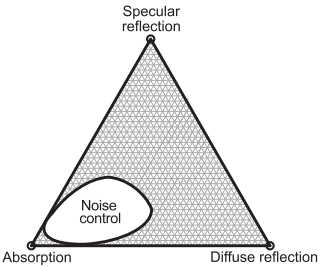
\includegraphics[width=0.7\textwidth]{Chapter-1/figs/noisecontrol}
    \caption{Breakdown of Noise Control \cite{Cox2004}}
    \label{fig:noisecontrol}
\end{figure}

\clearpage

Usually, acoustic absorption is broken down into two types. These are active absorption and passive absorption. Generally, active noise control solutions perform better in low frequencies while passive noise control solutions perform better in higher frequencies as shown in Figure \ref{fig:passivevsactive}. Absorbing materials are passive mediums that lower noise by disseminating energy and turning energy into heat. In porous materials at high frequencies, an adiabatic process takes places that produces heat loss due to friction when the sound waves cross the uneven pores. At lower frequencies poroelastic materials absorb sound by energy loss caused by heat exchange. This is an isothermal process. This is why poroelastic materials are much more efficient at absorbing higher frequencies \cite{Sagartzazu2008}.
% Active vs. Passive frequency ranges
\begin{figure}[hbtp]
    \centering
    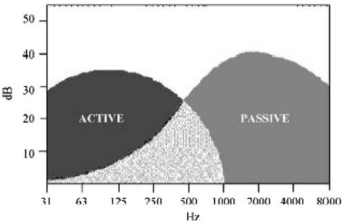
\includegraphics[width=0.6\textwidth]{Chapter-1/figs/passivevsactive}
    \caption{Active vs. Passive Noise Control frequencies \cite{Sagartzazu2008}}
    \label{fig:passivevsactive}
\end{figure}

Figure \ref{fig:activeNoiseComplex} shows an automotive application control system. However, it is noted that these systems require input energy and are generally very complex \cite{Shoureshi1996}. Passive techniques are generally used in architectual spaces as can be seen in Figure \ref{fig:woodabsorption} and Figure \ref{fig:concerthall}.

% Active Noise Canceling Automotive application Figure!
\begin{figure}[hbtp]
    \centering
    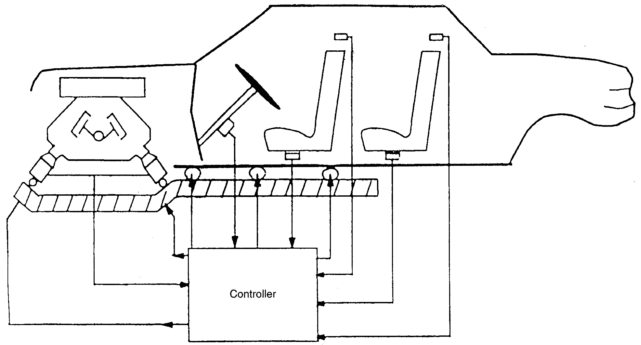
\includegraphics[width=0.8\textwidth]{Chapter-1/figs/activeNoiseComplex}
    \caption{Active Noise Control Application - Automotive \cite{Shoureshi1996}}
    \label{fig:activeNoiseComplex}
\end{figure}

% Passive Example 1
\begin{figure}[hbtp]
    \centering
    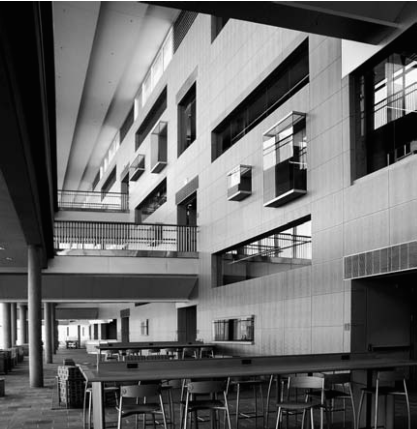
\includegraphics[width=0.5\textwidth]{Chapter-1/figs/woodabsorption}
    \caption{Passive Application - Wooden Architecture \cite{Cox2004}}
    \label{fig:woodabsorption}
\end{figure}

% Passive Example 2
\begin{figure}[hbtp]
    \centering
    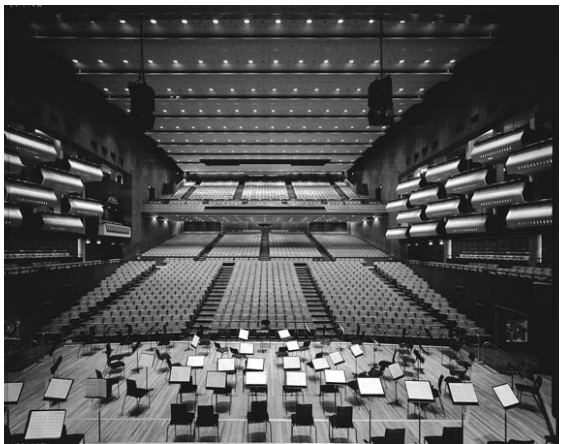
\includegraphics[width=0.55\textwidth]{Chapter-1/figs/concerthall}
    \caption{Passive Application - Concert Hall \cite{Cox2004}}
    \label{fig:concerthall}
\end{figure}

\clearpage

\subsection{Cellulose Acetate}
Cellulose Acetate is the acetate ester of cellulose. Figure \ref{fig:celluloseacetatestructure} shows the chemical structure of Cellulose Acetate. Cellulose Acetate is made by combining cellulose (cotton) and acetic acid. \cite{Welch1924} Cellulose Acetate can be manufactured with various filler materials, and made into different forms. Since cellulose acetate is such a basic chemical, it has a variety of uses outside of acoustics. A commonly known form of cellulose acetate with a TiO$_{\text{2}}$ filler manufactured into rods is the material used in cigarette filters.

% Cellulose Acetate Structure Figure!
\begin{figure}[hbtp]
    \centering
    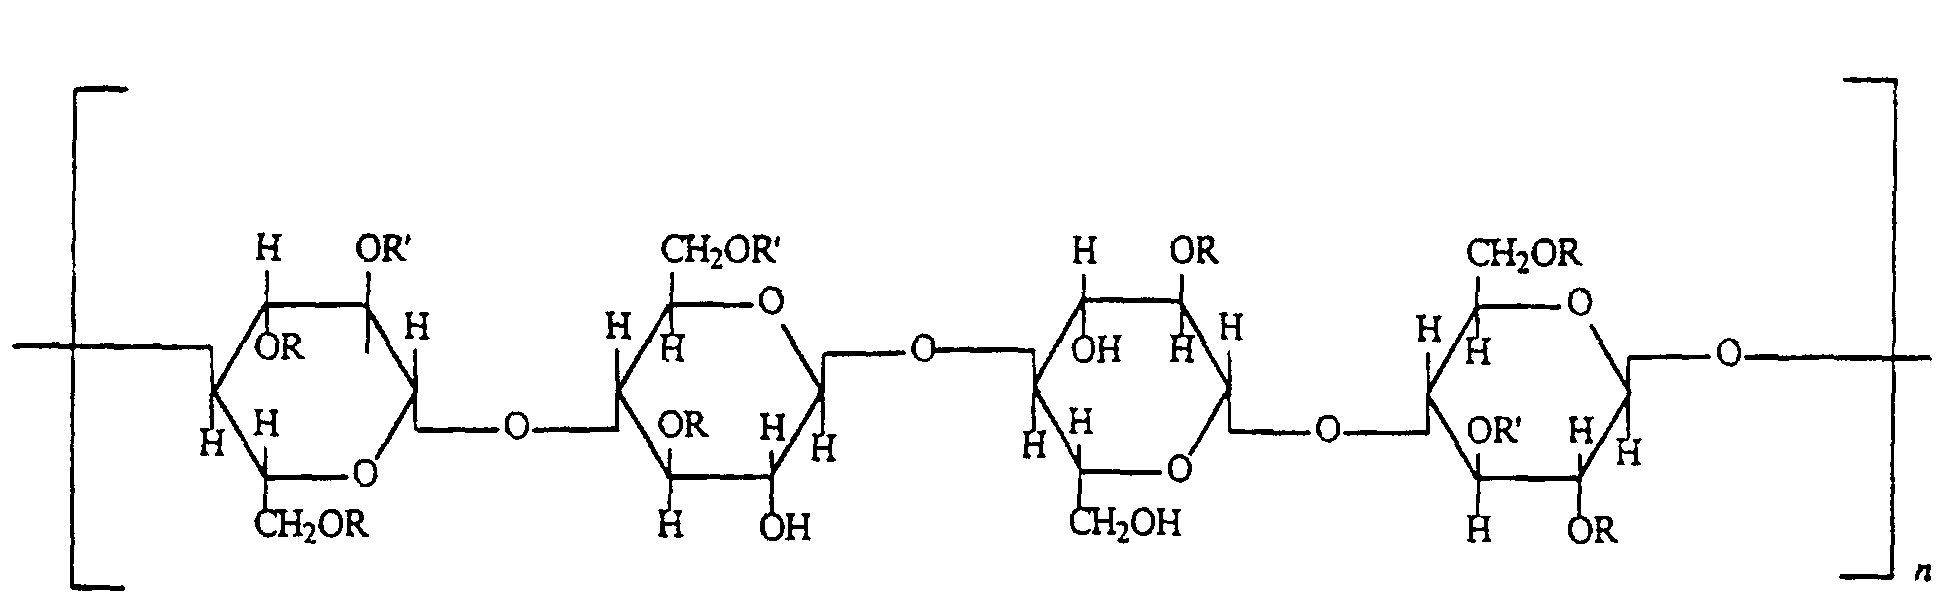
\includegraphics[width=1\textwidth]{Chapter-1/figs/celluloseacetatestructure}
    \caption{General Structure of Cellulose Acetate}% \cite{CA}}
    \label{fig:celluloseacetatestructure}
\end{figure}

\clearpage

Porous materials come in many varieties as shown in Figure \ref{fig:soundabsorbingmaterials}. Parts a) and b) show an SEM image of acoustic foams. Parts c) and d) show fibrous type materials. Cellulose Acetate is able to be manufactured into either of these microstructures.

% Sound absorbing materials Figure!
\begin{figure}[hbtp]
    \centering
    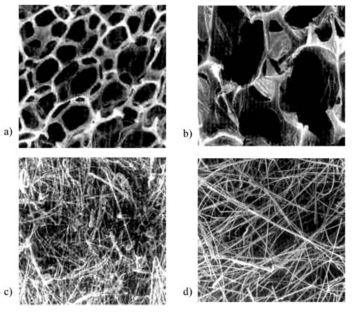
\includegraphics[width=0.8\textwidth]{Chapter-1/figs/soundabsorbingmaterials}
    \caption{Structures of different porous materials: (a) Reticulated foam (b) Partial reticulated foam (c) Mineral Wool (d) Fiberglass \cite{Sagartzazu2008}}
    \label{fig:soundabsorbingmaterials}
\end{figure}

\section{Biocompatibility}

For a new sound absorption material to be competitive in the currently dominated sound absorption market, it must present some novelty. A material that is biologically friendly enables new applications for the control of sound in rooms. Cellulose Acetate has been investigated and does not present health concerns. \cite{Liu2002} \cite{Nguyen2013} \cite{Welch1924} \cite{Zeng2009} 

It is important to note that the Cellulose Acetate Tow used in the experiments in this paper has a TiO$_{\text{2}}$ filler material used in it as manufactured by Eastman Chemical Company. It has been noted by \cite{Welch1924} that it is possible to make Cellulose Acetate with other hazardous chemicals, however the filler TiO$_{\text{2}}$ is not one of these. Therefore the Cellulose Acetate used in the experiments in this paper is biologically friendly.

\section{Previous Work}

Much research in the field of understanding how porous materials function for sound absorption has occurred. Due to the complex nature of the problems, empirical relationships have been developed. Similarly, an investigation into the poroelastic parameters controlling the absorption has occurred. Chapter \ref{chap-two} will discuss previous work in the field of porous absorption, as well as, develop the required equations as they relate to Cellulose Acetate absorption.

\section{Research Objectives}
The objective of this research is to present an investigation of Cellulose Acetate Tow for use as an acoustic absorption material. Figure \ref{fig:impedancetube} shows the experimental equipment used in the experiment designed to analyze Cellulose Acetate Tow's acoustic performance.

% Impedance Tube Figure!
\begin{figure}[hbtp]
    \centering
    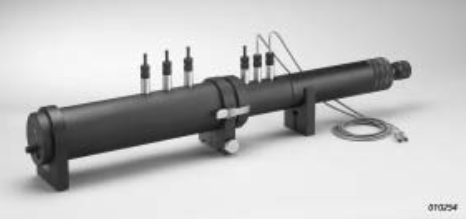
\includegraphics[width=0.7\textwidth]{Chapter-1/figs/impedancetube}
    \caption{Br�el \& Kj�r Impedance/Transmission Loss Measurement Tubes Type 4206A \cite{Kjaer2011}}
    \label{fig:impedancetube}
\end{figure}





\chapter{THEORY}
\label{chap-two}

\section*{Theory}

This chapter contains the necessary mathematical background a well as review of current literature related to research in the theory of absorption in porous media.

\section{Background Equations and Definitions}

This section focuses on the background equations and relevant definitions. Basic equations and theory are pulled from \cite{Kinsler1999}.

\subsection{Basic Vibration Definitions}
At the most basic level, any vibration problem involves frequency. Frequency is defined as the number of cycles per second in Hz. For an oscillatory system, frequency is defined as:
\begin{equation}
	f = \frac{2\pi}{\omega_0} = \frac{1}{T}
\end{equation}
The goal of energy is to get waves to dissipate. Whenever a real body is set into oscillation, dissipative (frictional) forces arise. Depending on the type of oscillating system, the oscillations will damp with respect to time. The viscous frictional force, $F_r$, on a simple oscillating system is expressed as
\begin{equation}
	F_r = -R_m\frac{dx}{dt}
\end{equation}
where $R_m$ is a positive constant called mechanical resistance of the system.
Sometimes materials reach a certain value, resulting in resonance. This occurs when mechanical reactance $X_m$ vanishes and the mechanical impedance is purely real with its minimum at $Z_m = R_m$. 

\subsection{Wave Equation}
At the heart of any acoustics problem is the wave equation. To develop the wave equation, a few formulas are required.
The thermodynamic speed of sound in fluids is defined as
\begin{equation}
	c^2 = ( \frac{\partial P}{\partial \rho} )_{adiabat}
\end{equation}
which corresponds to a value of $c_0 = 331.5 \text{m/s}$ for air at room temperature. For acoustics problems, the fluid is air, however, the theory holds true for other fluids with different constant values associated with them. The speed of sound can also be expressed as a perfect gas as defined as
\begin{equation}
	c^2 = \gamma r T_K
\end{equation}
The value $r$ depends on the universal gas constant $R$ and the molecular weight $M$ of the particular gas, which for air $r \approx 287  \text{J/(kg} \centerdot \text{K})$. 
This leads to the Equation of State, which for a perfect gas is defined as
\begin{equation}
	P = \rho r T_K
\end{equation}
where $P$ is total pressure in pascals, $\rho$ is the density in kilograms per cubic meter, and $T_K$ is the absolute temperature in kelvins.
The Equation of continuity is defined as:
\begin{equation}
	\frac{\partial s}{\partial t} + \nabla \centerdot \overrightarrow{u} = 0
\end{equation}
Euler's Equation is defined as
\begin{equation}
	\rho_0 \frac{\partial \overrightarrow{u}}{\partial t} = - \nabla p
\end{equation}
Combining the Equation of State, Continuity Equation, and Euler's equation yields the Wave Equation. For one dimension the general wave equation is the following:
\begin{equation}
	\frac{\partial^2 y}{\partial x^2} = \frac{1}{c^2} \frac{\partial^2 y}{\partial t^2}
\end{equation}
where the constant $c^2$ is defined as
\begin{equation}
	c^2 = \frac{T}{\rho_L}
\end{equation}
The wave equation can be linearized and expressed as the linear wave equation which is defined as
\begin{equation}
	\nabla^2 p = \frac{1}{c^2} \frac{\partial^2 p}{\partial t^2}
\end{equation}
Various researchers have discussed the wave equation as it applies to porous media \cite{Graber2012}. Graber developed a model of the semilinear porous acoustic boundary conditions with nonlinear boundary/interior sources and a nonlinear boundary/interior damping.
\subsection{Specific Acoustic Impedance}
Specific acoustic impedance is the ratio of acoustic pressure to the associated particle speed in a medium and is defined as
\begin{equation}
	z = p/u
\end{equation}
or when expressed solely for plane waves is defined as
\begin{equation}
	z = \rho_0 c
\end{equation}
In general, this is the complex of the form as defined as
\begin{equation}
	z = r + j x	
\end{equation}
where $r$ is the specific acoustic resistance, $x$ is the specific acoustic reactance of the medium for the particular wave being considered and $j$ is $\sqrt{-1}$.
Many acoustic properties rely on the specific acoustic impedance. It is possible to find the impedance $z$ at any angle $\theta$, however the impedance as defined normal to the surface $z_n$ is commonly used.
\begin{equation}
	\mathbf{z_n} = \frac{\mathbf{p}}{\mathbf{u} \cos \theta_i}
\end{equation}
\begin{equation}
	\mathbf{z_n} = \frac{r_1}{\cos \theta_i} \frac{1+\mathbf{R}}{1-\mathbf{R}}
\end{equation}
\begin{equation}
	\mathbf{R} = \frac{\mathbf{z_n} - r_1/\cos \theta_i}{\mathbf{z_n} + r_1/\cos \theta_i}
\end{equation}
\begin{equation}
	\mathbf{z_n} = r_n + j x_n
\end{equation}
For practical purposes, a low value of acoustic impedance is thought of as 'soft', while a high acoustic impedance is thought of as a 'hard' surface \cite{Bolt1944}.\\
\clearpage
\subsection{Decibel Scales}
Acoustic Intensity $I$ is defined as
\begin{equation}
	I = P_e^2 / \rho_0 c
\end{equation}
where $P_e = P/\sqrt{2}$.

Decibel levels are measured relative to a reference level. Commonly used references are intensity level, $IL$ and sound pressure level, $SPL$.\\
Intensity level, $IL$ is
\begin{equation}
	IL = 10 \log{I/I_{ref}}
\end{equation}
and sound pressure level, $SPL$ is
\begin{equation}
	SPL = 20 \log{P_e/P_{ref}}
\end{equation}

\subsection{Reflection of Waves}
Reflection occurs when a wave hits a solid surface and has some of the incident energy return. In Figure \ref{fig:reflectionWaves}, $p_i$ is the incident wave, $p_r$ is the reflected wave, and $p_t$ is the transmitted wave.
% Reflected Waves figure 1
\begin{figure}[hbtp]
    \centering
    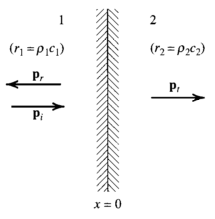
\includegraphics[width=0.35\textwidth]{Chapter-2/figs/reflectionWaves}
    \caption{Reflected Pressure Wave \cite{Kinsler1999}}
    \label{fig:reflectionWaves}
\end{figure}

The amount of energy reflected can be found by calculating the normal incidence reflection coefficient $R$
\begin{equation}
	\mathbf{R} = \frac{(r_n-r_1)+j x_n}{(r_n+r_1)+j x_n}
\end{equation}
However, any angle $\theta$ can be used by applying Snell's Law
\begin{equation}
	\frac{\sin \theta_1}{\sin \theta_2} = \frac{v_1}{v_2}
\end{equation}
which provides reflection coefficient generally as
\begin{equation}
	\mathbf{R} = \frac{(r_n-r_1/\cos \theta_i)+j x_n}{(r_n+r_1/\cos \theta_i)+j x_n}
\end{equation}

\subsection{Absorption}
The absorption coefficient is defined as
\begin{equation}
	\alpha = \sum_{i} \alpha_i
\end{equation}
where $\alpha_i$ represents each of the individual loss mechanisms calculated as if they were alone. The classical absorption coefficient $\alpha_c$ is the sum of the viscous and thermal absorption coefficients under the stokes assumption $\eta_B = 0$ and is defined as
\begin{equation}
	\alpha_c = \frac{\omega^2}{2\rho_0 c^3} \big(\frac{4}{3} + \frac{(\gamma - 1)\kappa}{c_P}\big)
\end{equation}

Mathematical formulation for calculating values is useful, however porous materials are complex by nature. Therefore, there are many formulas that are 'common sense' for acoustic engineers that are used in practice \cite{Bolt1944}. As a result, empirical equations for porous materials were developed by Biot \cite{Biot1962}.
The first experiments to calculate the absorption coefficient were carried out by Wallace C. Sabine in 1896 \cite{Bolt1944}. Sabine is credited with creating reverberation theory and the formula
\begin{equation}
	T = KV/\sum \alpha_j S_j
\end{equation}
The Eyring formula is the average absorption coefficient.
\begin{equation}
	\alpha = \sum \alpha_i S_i / \sum S_i
\end{equation}
The Eyring theory assumes that the energy in the room resumes uniform distribution after each set of incidences, and during the distribution after each set of incidences. All reverberation theory discussed is the energy lost at the walls. Rawlins \cite{Rawlins1983} corrected a small error made in formulation in \cite{Bolt1944}.

\section{Fiber Parameters}
Cellulose Acetate provided is a fibrous material and has some associated parameters that require definition.
\subsection{Total Denier}
Total Denier is the mass of a textile in grams per $9000$ meters. $1$ Denier is equivalent to $9000$ meters of fiber weighing $1$ gram.
\subsection{Denier per Filament (DPF)}
Denier per Filament (DPF) is defined as total denier divided by quantity of uniform filaments or 
\begin{equation}
	DPF = \frac{\text{Total Denier}}{\text{Quantity of uniform filaments}}
\end{equation}
\subsection{Fiber Cross Section}
Each fiber may have a different shape in its cross section. For experimental purposes in this paper, circular, X, Y and 8 legged cross sections were studied.  Table \ref{tab:crossSection} shows the fiber cross section.

\section{Chemical Relationships}
Cellulose Acetate is a polymer. A polymer is a chemical compound that is primarily composed of large quantities of similar repeating units. Polymers can be organic or inorganic, however, Cellulose Acetate is organic in structure \cite{Corsaro1990}.
A polymer's complex modulus is defined as:
\begin{equation}
	E^{*} = E' + iE''
\end{equation}
Where $E'$ is the storage modulus and $E''$ is the loss modulus.
The loss tangent is defined as:
\begin{equation}
	\tan{\delta} = E'' / E'
\end{equation}
The quantities $E''$ and $\tan{\delta}$ are of interest for absorption. Maximizing these parameters at a given frequency $f$ is the goal to maximize the absorption qualities of the material. It is important to note that with respect to frequency, $\tan{\delta}$ peaks at a higher temperature than $E''$ therefore making an optimal solution difficult to find as can be seen in Figure \ref{fig:tandelta}.
% Tan delta figure here
\begin{figure}[hbtp]
    \centering
    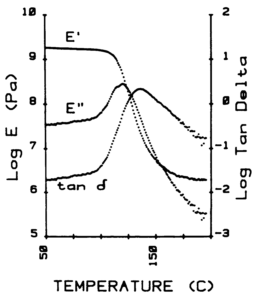
\includegraphics[width=0.4\textwidth]{Chapter-2/figs/tandelta}
    \caption{Typical Rheovibron data for polystyrene \cite{Corsaro1990}}
    \label{fig:tandelta}
\end{figure}

Temperature plays a role in the chemical reactions that result in porous absorption. The glass transition temperature of a polymer defined as $T_g$. The five regions of viscoelastic behavior can be found in Figure \ref{fig:viscoelasticregions}

% Viscoelastic Regions
\begin{figure}[hbtp]
    \centering
    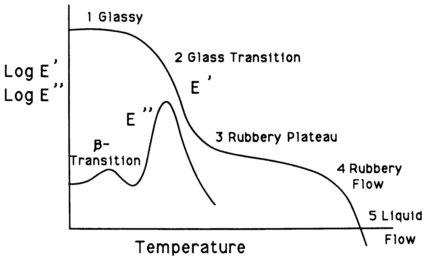
\includegraphics[width=0.7\textwidth]{Chapter-2/figs/viscoelasticregions}
    \caption{The five Viscoelastic Regions \cite{Corsaro1990}}
    \label{fig:viscoelasticregions}
\end{figure}

The key variables for damping are $T_g$, $E'$, $E''$, and $\tan{\delta}$

\section{Poroelastic Parameters}
Due to the complicated nature of absorption in porous materials, empirical methods have been developed \cite{Saint-Macary2006}. Viscoelastic porous materials are considered in a system of equations \cite{Shamaev2012}. Many of these methods rely on poroelastic parameters which have had much research in their identification \cite{Jaouen2008}. However, fibrous materials usually have no identifiable linear region, making these values difficult to measure \cite{Jaouen2008}. Fibers are usually layered causing materials to be anisotropic, however most materials are sufficiently homogenous for practical purposes and by only considering plane-wave propagation the isotropy requirement may be relaxed \cite{Delany1970}. Advances in technology are making it possible to run rather computationally intensive models to predict the properties of these kinds of waves in porous materials \cite{Mosanenzadeh2015}.\\
\indent The parameters can be broken down into fluid properties, structural properties, and fluid/structure interaction properties. This relies on the assumption made by Biot \cite{Biot1962} that sound traveling through porous material can be broken down into two categories; the fluid properties and the mechanical properties.

\subsection{Fluid Properties}
These properties relate to the behavior of the fluid as it travels through the porous object \cite{Sagartzazu2008}.\\
Volume Mass,
\begin{equation}
	\rho_0
\end{equation}
The Ratio of Specific Heats,
\begin{equation}
	\gamma = C_P/C_V
\end{equation}
Sound Velocity,
\begin{equation}
	c = \sqrt{\frac{\partial{\hat{p}}}{\partial \rho} (\rho_0, s_0)}
\end{equation}
where $c_0 = 331.5 \text{ m/s}$\\
Dynamic Viscosity,
\begin{equation}
	\eta = 1.72 x 10^{-5} \qquad \text{Pa $\centerdot$ s @ 0$^{\circ}$ C}
\end{equation}
Prandtl Number,
\begin{equation}
	P_r = \frac{\eta/\rho}{\kappa/\rho C_P} = \frac{\eta C_P}{\kappa}
\end{equation}
where the $P_r$ of air at $0^{\circ} \text{C}$ is equal to $0.708$
\subsection{Structural Properties}
These properties relate to the skeleton structure of the porous material \cite{Sagartzazu2008}
\begin{enumerate}
	\item Youngs Modulus, $E$
	\item Shear Modulus, $G$
	\item Poisson's Ratio, $\nu$
\end{enumerate}
\subsection{Fluid and Structural Interaction Properties}
These properties help define how the fluid and structural properties interface with one another \cite{Mosanenzadeh2015}.\\
Porosity,
\begin{equation}
	\phi = \frac{V_a}{V_t}
\end{equation}
Static Flow Resistivity,
\begin{equation}
	\sigma = \frac{8\eta}{\phi R^2}
\end{equation}
or,
\begin{equation}
	\sigma = E_1 \frac{7 \eta \alpha_{\infty}}{\phi R^2} (R_w)^{E_2} = E_1 \sigma' (R_w)^{E_2}
\end{equation}
Three non-acoustic properties:\\
Tortuosity,
\begin{equation}
	\alpha_{\infty} = \frac{\langle v_m^2 (N) \rangle _v}{v^2 (N_0)}
\end{equation}
The value of tortuosity is an intrinsic property of the porous frame that depends on the micro-geometry \cite{Mosanenzadeh2015}. Effective density of fluid $\rho$ is related to tortuosity by 
\begin{equation}
	\rho = \alpha_{\infty} \rho_0
\end{equation}
Viscous Characteristic Length,
\begin{equation}
	\Lambda = 2 \frac{\int_V v_i^2 (r) dV}{\int_A v_i^2 (r_w) dA}
\end{equation}
Thermal Characteristic Length,
\begin{equation}
	\Lambda' = \frac{2V_f}{A} = \frac{2l^3}{A_s(1-R_w)+(A_t-A_s)R_w}
\end{equation}
A fluid equivalent is based off of the Johnson-Champoux-Allard model.

\section{Empirical Models}
Due to complex expressions and the complex nature of porous materials, it is difficult to provide physical insight into the acoustic behavior of porous materials. It is also difficult to determine the dominate mechanism for sound absorption for a given material at a given frequency, $f$ \cite{Brennan2001}. There are currently two positions on prediction of acoustic properties of rigid-frame porous materials. One states that there are simple empirical expressions for noise control engineers to use and apply to predict the performance of porous material. Academic literature suggests relatively complicated expressions.\\
\indent The complicated expressions from academic literature often times require knowledge of many parameters of a material which is difficult to measure accurately. This also results in difficulty in determining which are the dominating physical traits of a material.\\
\indent Biot developed a model of mechanics of deformation and acoustic propagation in porous materials\cite{Biot1962}. Biot's model relies on the assumption that a porous material can be broken down into a fluid part and a solid part. This is the basis for many empirical models that have been based off of Biot's work. Generalized theory can be found in \cite{Biot1962a}. Dazel considers a porous elastic matrix as a fluid-saturated and statistically isotropic material. This work brings forth a general correspondence principle by which known results for elastic media may be immediately extended to the case of viscoelasticity by substituting operators for the elastic coefficient. Many authors have extended this work to generalize his theory \cite{Dazel2007} \cite{Albers2012}. Some newer equations have resulted in improved performance of the model in the lower frequency range \cite{Allard1992}.\\
\indent However, some authors still would like to reduce the complicated nature of the equations and bridge the gap between the complex expressions presented in academic literature and simplified expressions practically used  \cite{Brennan2001}. Brennan takes note that the effects of thermal losses are negligible in most situations and an upper bound on the thermal losses can be derived.\\
\indent A rigid local reacting porous material has two characteristics that describe its behavior. These are the acoustic wave number $k_c$ and the characteristic acoustic impedance $Z_c$.
\begin{equation}
	k_c = \omega \Big(\frac{\rho_e}{B_e}\Big)^{\frac{1}{2}}
\end{equation}
\begin{equation}
	Z_c = (\rho_e B_e)^{\frac{1}{2}}
\end{equation}
where $\rho_e$ and $B_e$ are the effective density and bulk modulus of the fluid contained within the porous material respectively.\\
\indent To approximate $\phi_e$ and $B_e$ the following expressions have been derived \cite{Brennan2001}
\begin{equation}
	\rho_e = \rho_0 \alpha_{\infty} \bigg( 1 + j \frac{\eta \phi}{\rho_0 \alpha_{\infty} k_0 \omega} \Big( 1 - j \frac{4\rho_0 \alpha_{\infty}^2 k_0^2 \omega}{\eta \phi^2 \Lambda^2} \Big) \bigg)
\end{equation}
\begin{equation}
		B_e = \frac{\gamma P}{\gamma - (\gamma - 1) \bigg( 1 + j \frac{\eta \phi}{\rho_0 Pr k'_0 \omega} \Big( 1 - j \frac{4 \rho_0 Pr k'_0 \omega}{\eta \phi^2 \Lambda'^2} \Big) ^{\frac{1}{2}} \bigg)^{-1}}
\end{equation}

Delany and Bazley's empirical model estimates the value of the propagation constant $jk_C$ and characteristic impedance $Z_C$ as a function of material flow resistivity. This model assumes that the material is fibrous and that the fibers are uniformly distributed. However, this only works well in a specific frequency range \cite{Sagartzazu2008}.
% these are emprical equations from Delaney and Bazley
\begin{equation}
	\rho_1/\rho = (\vert \rho_1 \vert / \rho) \exp {j \phi} = \mathbf{kW}/\rho \omega
\end{equation}
\begin{equation}
	\kappa / \gamma \mathbf{P} = (\vert \kappa \vert / \gamma \mathbf{P}) \exp {j \theta} = \omega W/k \rho c^2
\end{equation}
\begin{equation}
	W = \rho c [1 + 0.0571 X^{-0.754} - j0.087 X^{-0.732}]
\end{equation}
\begin{equation}
	k = (\omega/c)[(1+0.0978X^{-0.700}) - j0.189X^{-0.595}]
\end{equation}
where the frequency parameter is
\begin{equation}
	X = \rho f/R_1
\end{equation}

Delaney and Bazley suggest bounds for the validity of the empirical equation on the parameter $X$ as follows:
\begin{equation}
	0.01 < X < 1.0
\end{equation}

The Mechel-V�r model is a more refined adjustment than the Delany and Bazley model. It differentiates two families of absorption materials, and two areas for normalized adimensional parameters that are called the normalized frequency parameter, $E = \rho_0 f / \sigma$

\begin{equation}
	Z_C = \rho_0 c(1 + b' E^{-\beta'} - jb'' E^{-\beta''})
\end{equation}
\begin{equation}
	\Gamma_c = \frac{\omega}{c}[a' E^{-\alpha'} + j(1 + \alpha'' E^{-\alpha''}) ]
\end{equation}
that is
\begin{equation}
	k_C = -j \frac{\omega}{c} [a' E^{-\alpha'} + j(1 + \alpha'' E^{-\alpha''})]
\end{equation}
This model is even more accurate at lower frequencies than the Delany-Bazley model.\\
\indent Another recent empirical model that has been developed is the Allard-Champoux model. This model assumes that the thermal effects depend on the frequency. This model currently shows better results at low frequencies than all previous models. This model defines dynamic density and the compressibility modulus as follows:
\begin{equation}
	\rho(\omega) = \rho_0 \Big[1 - j \Big( \frac{\sigma}{\rho_0 \omega} \Big) G_1 \Big( \frac{\rho_0 \omega}{\sigma} \Big) \Big]
\end{equation}
\begin{equation}
	K(\omega) = \gamma P_0 \Big( \gamma - \frac{\gamma - 1}{1 - (\frac{j}{4 P_r}) (\frac{\sigma}{\rho_0 \omega}) G_2 (\frac{\rho_0 \omega}{\sigma})} \Big)^{-1}
\end{equation}
where $G_1(\rho_0 \omega/\sigma)$ and $G_2 (\rho_0 \omega/\sigma)$ are defined as
\begin{equation}
	G_1 \Big( \rho_0 \omega/\sigma \Big) = \sqrt{1 + \frac{j}{2} \bigg( \rho_0 \omega/\sigma \bigg)}
\end{equation}
\begin{equation}
	G_2 \Big( \frac{\rho_0 \omega}{\sigma} \Big) = G_1 \Big( \frac{\rho_0 \omega}{\sigma} \Big) \Big( 4 P_r \Big( \frac{\rho_0 \omega}{\sigma} \Big) \Big)
\end{equation}
where $P_0$ is the balance pressure.

With many different models available, Figure \ref{fig:empiricalcomparisons} shows that many of the empirical modeling techniques adherer to experimental data well.
% Empirical Comparisons
\begin{figure}[hbtp]
    \centering
    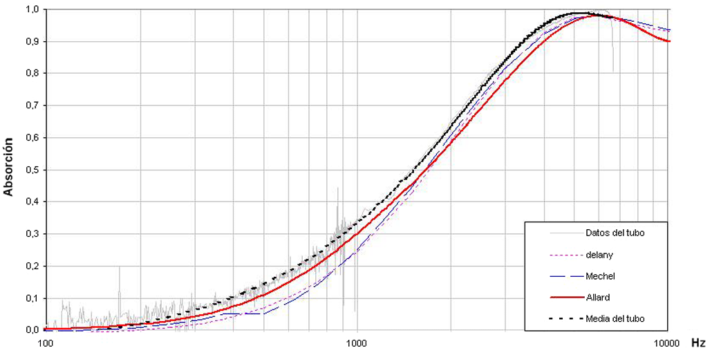
\includegraphics[width=1\textwidth]{Chapter-2/figs/empiricalcomparisons}
    \caption{Comparison of Empirical Approximations on wool type material \cite{Sagartzazu2008}}
    \label{fig:empiricalcomparisons}
\end{figure}
\clearpage

Many authors have taken the results of the work by Biot et al. to use in their in their own research applications. Topics range from Helmholtz resonators \cite{Boutin2013}, to finite-element modeling \cite{Atalla2001}, \cite{Rumpler2012}, \cite{Kook2014}, to the scattering effect of non-porous materials \cite{Velea2001}, to Rayleigh attenuation \cite{Bouhedja2011}, and to various other acoustic materials \cite{Voronina1998} \cite{Voronina1999} \cite{Biot1934}.

\section{Measurement Techniques}
Measurement of acoustic parameters is of interest \cite{Gayathri2013}, \cite{Horoshenkov2001}. The empirical models rely on the ability to accurately measure parameters about the test sample. Many techniques have been developed to obtain these values.

\subsection{Flow Resistance}
The flow resistance of a material plays a large role in an open cell porous material's ability to interface with sound \cite{Ingard1985}. Flow resistance can be measured using a two-channel analyzer. The normalized flow resistance is the absolute value of the imaginary part of the pressure ratio, or $\theta = \vert \operatorname{Im}(p_1/p_3) \vert$. At low frequencies the flow reactance is small compared to the resistance and can be approximated by $\theta = \vert p_1/p_3 \vert$.
Normalized flow reactance is as follows
\begin{equation}
	\chi = (-1)^{n-1} \operatorname{Re}(p_1/p_3)
\end{equation}

Other calculations relying on the Kozeny number \cite{Lambert1984} or reflected waves \cite{Sebaa2005} to find static flow resistance also are valid. Figure \ref{fig:flowresistancemeasurement} shows a device used by Bies.

% Flow Resistance Measurement Device
\begin{figure}[hbtp]
    \centering
    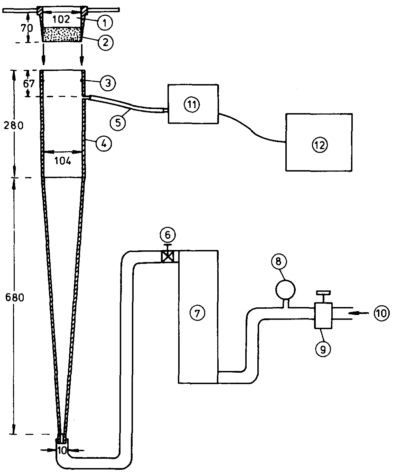
\includegraphics[width=0.45\textwidth]{Chapter-2/figs/flowresistancemeasurement}
    \caption{Flow Resistance Measurement Device \cite{Bies1980}}
    \label{fig:flowresistancemeasurement}
\end{figure}

\subsection{Tortuosity}
Allard developed a technique for the measurement of tortuosity in air saturated open cell porous sound absorbing materials. It is noted that it is difficult to obtain the measurement for some materials without damaging the sample material \cite{Allard1994}.

\subsection{Porosity}
% Measurement - Porosity
Porosity is defined as the volume fraction of air contained in a material. This technique is based on the ideal gas law. \cite{Champoux1991}
\begin{equation}
	\phi = V_a/V_t
\end{equation}
where $V_a$ is the air filled volume and $V_t$ is the total volume. The total volume of air in the measurement chamber is $V' = V_0 + V_a$ where $V_0$ is the residual volume in the sample chamber outside of the sample. Figure \ref{fig:porositychamber} shows this test set up.
% Porosity chamber measurement figure !
\begin{figure}[hbtp]
    \centering
    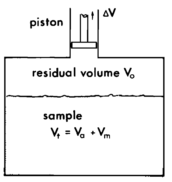
\includegraphics[width=0.4\textwidth]{Chapter-2/figs/porositychamber}
    \caption{Porosity Measurement Chamber}
    \label{fig:porositychamber}
\end{figure}
Then $V_a$ is calculated by
\begin{equation}
	V' = -[(P_0 + \Delta P')/ \Delta P'] \Delta V
\end{equation}
and air content is then
\begin{equation}
	V_a = V' - V_0
\end{equation}

To help determine the internal pore surface area per unit area of a solid, \cite{Leclaire1998} developed a technique for integrating the water extraction curve. This method works well for acoustic type materials to determine the specific area needed in previous calculations.

\subsection{Impedance}
Impedance measurement of porous materials is an important topic \cite{McGrath1952}. There are techniques developed by Allard for in situ measurement of acoustic surface impedance, which can provide valuable information when manufacturing acoustic absorption materials. A technique using two-microphones above the surface of which impedance is measured is detailed in \cite{Allard1989}, and again in \cite{Allard2003} for porous materials.

\subsection{Reflection Coefficients}

Tamara developed the technique for measuring reflection coefficient at oblique angles \cite{Tamura1990} and continued on in \cite{Tamura1995} with experimental results. The basic principle relies on decomposing spherical waves into plane waves by spatial Fourier transform. Decomposing spherical waves into plane waves is done by
\begin{equation}
	P(k_x,k_y,k_z) = \int \int_{-\infty}^{\infty} p(x,y,z_j) \exp{-i(k_x x + k_y y)} dx dy
\end{equation}
\begin{figure}[hbtp]
    \centering
    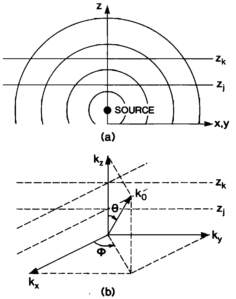
\includegraphics[width=0.5\textwidth]{Chapter-2/figs/sphericaltoplanewaves}
    \caption{Decompose Spherical Waves into Plane Waves}
    \label{fig:sphericaltoplanewaves}
\end{figure}

Solving this for incident and reflected pressure-wave components in the x-y plane we get the following expressions for $P_i$ and $P_r$
\begin{equation}
	P_i(k_x,k_y,0)  = \frac{P(k_x,k_y,z_1)\exp{i k_z z_2} - P(k_x,k_y,z_2) \exp{i k_z z_1}}{2 i \sin{k_z (z_2 - z_1)}}
\end{equation}
\begin{equation}
	P_r(k_x,k_y,0) = \frac{P(k_x,k_y,z_2)\exp{-i k_z z_2} - P(k_x,k_y,z_1) \exp{-i k_z z_1}}{2 i \sin{k_z(z_2 - z_1)}}
\end{equation}
where coefficient of reflection $C_r$ is defined as the ratio between the reflected and incident pressure waves
\begin{equation}
	C_r(k_x,k_y) = P_r(k_x,k_y,0) / P_i(k_x,k_y,0)
\end{equation}

This theory has been modeled using the reflection coefficient of absorbing materials measured from an impedance tube for normal sound incidence \cite{Lanoye2006}. The Tamara method can determine the angle dependency of the surface impedance and the absorption coefficient. The Tamura technique measures sound pressure in two planes parallel to the surface of interest, and a 2d Fourier transformation is used to calculate the angle dependent surface impedance.

In a standing wave tube the sound pressure at a distance $x$ from the rigid ending is given by
\begin{equation}
	p(x,t,\omega) = A(\exp{ikx}+\exp{-ikx})\exp{-i\omega t}
\end{equation}
and the particle velocity at the same distance is defined by
\begin{equation}
	u(x,t,\omega) = \frac{1}{i\omega \rho_0} \frac{\partial p(x,t,\omega)}{\partial x} = \frac{A}{\rho_0 c} (\exp{ikx} - \exp{-ikx}) \exp{-i \omega t}
\end{equation}
These values are calculated in real time using a well calibrated velocity-pressure transducer. From this knowledge the value of the surface impedance can be calculated for normal to slightly oblique incidence. Figure \ref{fig:reflectionWavesrelatedAbsorption} shows that pressure reflection coefficient is inversely proportional to absorption coefficient.
% Reflected Waves figure 2
\begin{figure}[hbtp]
    \centering
    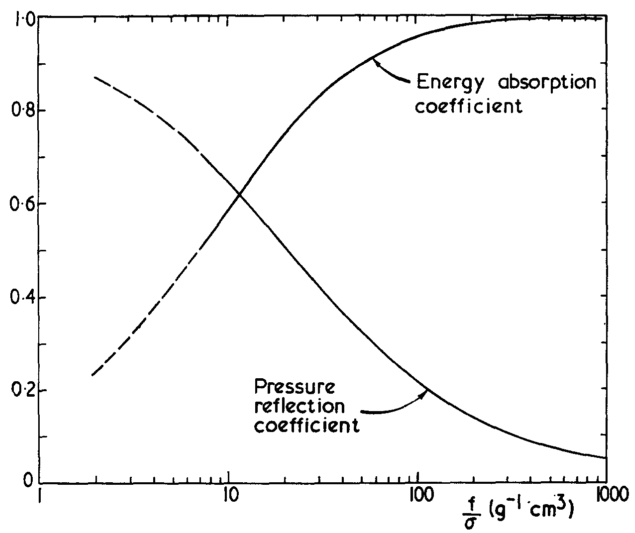
\includegraphics[width=0.7\textwidth]{Chapter-2/figs/reflectionWavesrelatedAbsorption}
    \caption{Reflected Pressure Coefficient Relation to Absorption \cite{Delany1970}}
    \label{fig:reflectionWavesrelatedAbsorption}
\end{figure}

\section{Impedance Tube Method Definition}

Referencing \cite{Kjaer2011} includes detailed information on how the Impedance tube system is able to calculate its value for absorption coefficient $\alpha$. Figures \ref{fig:impedancetube2} and \ref{fig:impedancetube3} show the system configuration.

% Testing set up 1
\begin{figure}[hbtp]
    \centering
    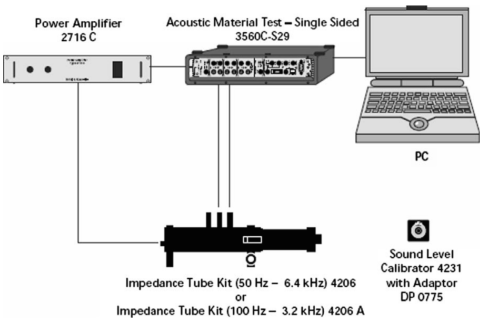
\includegraphics[width=0.95\textwidth]{Chapter-2/figs/impedancetube2}
    \caption{Impedance Tube Testing Set up \cite{Ersoy2009}}
    \label{fig:impedancetube2}
\end{figure}

% Impedance Tube Method
\begin{figure}[hbtp]
    \centering
    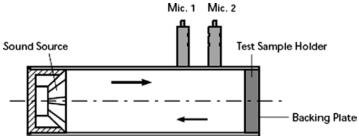
\includegraphics[width=0.75\textwidth]{Chapter-2/figs/impedancetube3}
    \caption{Impedance Tube Method \cite{Ersoy2009}}
    \label{fig:impedancetube3}
\end{figure}

The two-microphone system functions by decomposing the incident wave generated by the sound source into its incident and reflected components. From this information, the complex reflection coefficient $R$ is found by:
\begin{equation}
	R = \Bigg( \frac{H_1 - H_i}{H_r - H_1} \Bigg) \exp{j 2 k (l + s)}
\end{equation}
where $k$ is the wave number, $l$ is the distance from the first microphone to the front of the sample, $s$ is the distance between the two microphones, and $H$ are frequency response functions. $H_i$ corresponds to the incident component, $H_r$ corresponds to the reflected component and $H_1$ corresponds to the sample.

From the complex reflection coefficient, the system is able to find the normalized impedance ratio $(z/\rho c)$and absorption coefficient $\alpha$ by the following equations.

%normalied impedance ratio
\begin{equation}
	\frac{z}{\rho c} = \frac{1+R}{1-R}
\end{equation}
% sound absorption coefficient
\begin{equation}
	\alpha = 1 - \vert R \vert ^2
\end{equation}
It should be noted that two-microphone theory assumes plane-wave propagation, no mean flow, and no losses due to absorption at the tube wall. 

\subsection{Microphone Calibrations}
In order for the system to accurately find the frequency response functions $H$, each microphone must be properly calibrated by a calibration factor $H_C$ found by:
\begin{equation}
	H_C = \vert H_C \vert \exp{j \phi_C}
\end{equation}
where
\begin{equation}
	H_c = \sqrt{\vert H_{C1}\vert \vert H_{C2}\vert}
\end{equation}
\begin{equation}
	\phi_C = \frac{1}{2} (\phi_1 + \phi_2)
\end{equation}
where $\phi_1$ and $\phi_2$ are the phase of the calibration frequency response $H_C1$ and $H_C2$ respectively.
Applying this correction factor to $H_1$ yeilds
\begin{equation}
	H_1 = \frac{H}{H_C} = \vert H_1 \vert \exp{j \phi_h}
\end{equation}
where
\begin{equation}
	\phi_h = \phi - \phi_C
\end{equation}
Once this calibration is applied, the value $H_1$ is used to determine the acoustic properties of the test sample.

\subsection{Working Frequency Range}
The theoretical impedance tube system would span a relatively large frequency range, however in practice the working frequency range is much smaller. The working frequency range is defined by
\begin{equation}
	f_l < f < f_u
\end{equation}
The lower working frequency $f_l$ is limited. \cite{ISO1998}.
\begin{itemize}
	\item The $f$ resolution of the analysis system
	\item The $f$ response of the loudspeaker
	\item The spacing between the microphones
\end{itemize}
The upper working frequency $f_u$ is chosen to avoid the occurrence of non-plane wave mode propagation and to assure accurate phase detection \cite{Kjaer2011}. Various standards provide guidelines for the physical concerns of the system. \cite{ASTM1990}, \cite{ASTM2011}.

In order to maintain plane wave propagation, the upper frequency limit is defined as:
\begin{equation}
	f_u < K c / d \qquad \text{or} \qquad d < K c / f_u
\end{equation}
where $f_u$ is the upper frequency limit, $c$ is the speed of sound in the tube, $d$ is the diameter of the tube, and $K = 0.586$.

A large spacing between the microphones enhances accuracy of the measurements, however the spacing must be less than the shortest half-wavelength of interest.
\begin{equation}
	s << c / 2 f_u
\end{equation}
where $s$ is microphone spacing. It is recommended that s be $80\%$ of $c / 2 f_u$.

The length of the tube should be sufficiently long enough as to allow plane waves to fully develop before reaching the microphones and test specimen. A recommended minimum is three tube diameters between the sound source and the nearest microphone.

The specimens location relative to the closest microphone is ideally at a minimum, however the surface characteristics of the sample play a role. This distance can be modified as follows.
\begin{itemize}
	\item Flat Surface
	The closest microphone can be within one-half of the tube diameter.
	\item Nonhomogenous Surface
	The closet microphone can be at least one tube diameter in order to suppress higher order modes resultant of the non homogenous surface of the sample.
	\item Asymmetrical Surface
	The closest microphone can be at least two tube diameters to suppress higher order modes resultant.
\end{itemize}

For the Impedance Tube system used in the experiments in this paper, Table \ref{tab:workingfreq} shows the appropriate associated values.

% Landscape page of Samples from Eastman Chemical Company
\newgeometry{margin=1in,lmargin=1.25in,footskip=\chapterfootskip, includehead, includefoot}
    %\thispagestyle{lscape}
    %\pagestyle{lscape}
    \thispagestyle{lscapedplain}
    \begin{landscape}
	\begin{table}
    \caption{Working Frequencies of Impedance Tube}
    \label{tab:workingfreq}
    \begin{center}
    \begin{tabular}{lcl}
    \toprule
    Parameter & Large Tube Wide Spacing & Small Tube\\
    \midrule
    Tube Diameter (mm) & 100 & 29\\
    Microphone Spacing (mm) & 100 & 20\\
    Distance from Sample to Mic B (mm) & 100 & 35\\
    Distance from Source to Mic A (mm) & 100 & 370\\
    Provided Lower Frequency Limit (Hz) & 50 & 500\\
    Provided Upper Frequency Limit (Hz) & 1600 & 6400\\
    Calculated Lower Frequency Limit (Hz) & 34.3 & 171.5\\
    Calculated Upper Frequency Limit (Hz) (Based on Diameter) & 2010 & 6931\\
    Calculated Upper Frequency Limit (Hz) (Based on Microphone Spacing) & 1372 & 6860\\
    \bottomrule
    \end{tabular}
    \end{center}
	\end{table}
    \end{landscape}
    %\newgeometry{margin=1in,lmargin=1.25in,footskip=\chapterfootskip, includehead, includefoot,landscape=false}
    \restoregeometry
    \pagestyle{fancy}
    \thispagestyle{fancy}
\newgeometry{margin=1in,lmargin=1.25in,footskip=\chapterfootskip, includehead, includefoot}




\chapter{EXPERIMENTAL SETUP}
\label{chap-three}

\section*{Experimental Setup}

This chapter contains details regarding the set up of the experiment to measure absorption coefficients of various materials. The tests were performed in a Br�el \& Kj�r Impedance/Transmission Loss Measurement Tubes Type 4206A and the PULSE data acquisition software. Detailed instructions on use of the equipment can be found in Appendix \ref{append-B}.

\section{List of Materials}

\subsection{Cellulose Acetate Materials}
Many of the materials tested were provided by Eastman Chemical Company. They are as noted in the following list and as shown in Table \ref{tab:ECCsamples}. Table \ref{tab:crossSection} shows the fiber cross section.

% Small List of other materials from Eastman Chemical Company
\begin{enumerate}
    \item Several hundred white filter rods made with 2.5 DPF, Y Cross Section, 35000 total denier tow (2.5Y35000, Lot 2.5-258, tow manufactured 3/28/2014)
    \item A hand full of filter rods made with black tow
    \item A 6" by 12" sheet of cellulose acetate film made from CA-394-605 polymer
    \item Knitted Samples from Table \ref{tab:ECCsamples} below
\end{enumerate}

\begin{table}[htb]
        \caption{Fiber Cross Section Type}
        \label{tab:crossSection}
        \begin{center}
        \begin{tabular}{lcccccl}
        \toprule
        Fiber Cross Section Type & Image \\
        \midrule
        Circle & 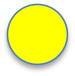
\includegraphics[width=0.07\textwidth]{Chapter-3/figs/circle} \\
        X & 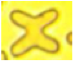
\includegraphics[width=0.07\textwidth]{Chapter-3/figs/x} \\
        Y & 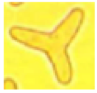
\includegraphics[width=0.07\textwidth]{Chapter-3/figs/y} \\
        8 Leg & 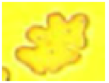
\includegraphics[width=0.07\textwidth]{Chapter-3/figs/eightleg} \\
        \bottomrule
        \end{tabular}
        \end{center}
\end{table}

% Landscape page of Samples from Eastman Chemical Company
\newgeometry{margin=1in,lmargin=1.25in,footskip=\chapterfootskip, includehead, includefoot}
    %\thispagestyle{lscape}
    %\pagestyle{lscape}
    \thispagestyle{lscapedplain}
    \begin{landscape}
    \begin{table}
        \caption{Eastman Chemical Company Samples}
        \label{tab:ECCsamples}
        \begin{center}
        \begin{tabular}{lcccccl}
        \toprule
        Sample Number & Composition & Total Denier & DPF & No. of Filaments & Fiber Cross Section\\
        \midrule
        EX1054-15-1-SOCK & Nylon & 200 & 5.9 & 34 & Round \\
        EX1054-15-2-SOCK & PET & 220 & 6.3 & 35 & Round \\
        EX1054-15-3-SOCK & Glass & 600 & 5 & 120 & Round \\
        \midrule
        EX1054-9-5-SOCK & Cellulose Acetate (TiO2) & 1576 & 2 & 788 & Y \\
        EX1054-9-1-SOCK & CA (TiO2) & 152 & 4 & 38 & Y \\
        EX1054-9-6-SOCK & CA (TiO2) & 1788 & 6 & 298 & Y \\
        EX1153-8-2-SOCK & CA (TiO2) & 1800 & 3 & 600 & Y \\
        EX1054-9-8-SOCK & CA (TiO2) & 170 & 2 & 85 & 8 Leg \\
        EX1054-9-9-SOCK & CA (TiO2) & 152 & 4 & 38 & 8 Leg \\
        EX1054-9-3-SOCK & CA (TiO2) & 150 & 6 & 25 & 8 Leg \\
        EX1054-18-1-SOCK & CA (no colorants) & 150 & 4 & 38 & 8 Leg \\
        EX1054-18-2-SOCK & CA (black colorant) & 150 & 4 & 38 & 8 Leg \\
        EX1054-18-3-SOCK & CA (TiO2) & 1800 & 4 & 450 & X \\
        EX1054-18-4-SOCK & CA (TiO2) & 1800 & 6 & 300 & X \\
        \bottomrule
        \end{tabular}
        \end{center}
    \end{table}
    \end{landscape}
    %\newgeometry{margin=1in,lmargin=1.25in,footskip=\chapterfootskip, includehead, includefoot,landscape=false}
    \restoregeometry
    \pagestyle{fancy}
    \thispagestyle{fancy}
\newgeometry{margin=1in,lmargin=1.25in,footskip=\chapterfootskip, includehead, includefoot}

% Figure of Socks from Eastman Chemical Company
\begin{figure}[hbtp]
    \centering
    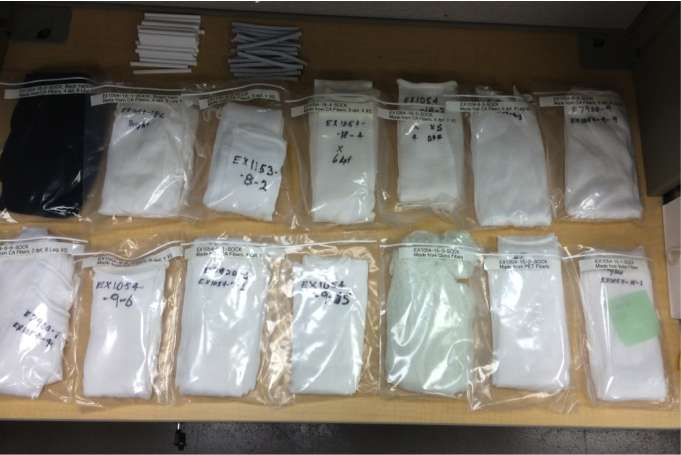
\includegraphics[width=1\textwidth]{Chapter-3/figs/ECCsocks}
    \caption{Sock Samples and Filter Rods provided by Eastman Chemical Company}
    \label{fig:ECCsocks}
\end{figure}

Above in Figure \ref{fig:ECCsocks} are all the Sock, Filter Rod, and Raw Tow materials provided by Eastman Chemical Company. Each part number provided different physical quality of Acetate Tow as shown in Table \ref{tab:ECCsamples}. 

\subsection{Commercial Materials}
In addition to Cellulose Acetate materials, commercial materials of various types were analyzed to compare to the Cellulose Acetate materials of similar type. The list of commercial materials tested is shown below.

\begin{enumerate}
	\item Sock Materials
		\begin{enumerate}
			\item Fiberglass Sock
			\item PET Sock
			\item Nylon Sock
		\end{enumerate}
	\item Raw Material Type
		\begin{enumerate}
			\item Raw Cotton Balls
			\item Auralex Compressed Cotton
		\end{enumerate}
	\item Acoustic Foam Type
		\begin{enumerate}
			\item Br�el \& Kj�r Foam
			\item Auralex Acoustics Foam
		\end{enumerate}
	\item Acoustic Panneling Type
		\begin{enumerate}
			\item Owens Corning Fiberglass Panel
			\item	Auralex Compressed Polyester Panel
		\end{enumerate}
\end{enumerate}

\section{Material Preparation for Testing}

\subsection{Sock Material Testing and O-ring}
The Sock type materials presented a challenge when testing impedance tube system. Due to the nature of the manufacture of the Sock, the materials would not lay flat on the testing surface without support. To appropriately support the woven sock type materials in the Impedance tube system, the materials were stapled to a 70-dura rubber O-ring. This method was found to be the best to prevent air gaps between the sample and the backing plate. The structural O-ring provided a means for the fabric materials to not 'curl up' in the testing area in order to get a proper measurement. This was done for each size of the Impedance tube system at 100mm and 29mm. The figure below shows a woven sock attached to the 100mm O-ring. 
\begin{figure}[hbtp]
    \centering
    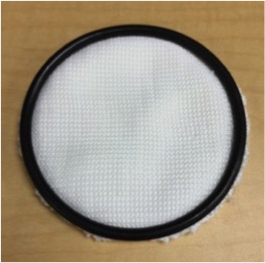
\includegraphics[width=0.4\textwidth]{Chapter-3/figs/sockOring}
    \caption{Sock Sample attached to 100mm O-ring}
    \label{fig:sockOring}
\end{figure}
In order to build a relationship regarding the thickness of the material, each Sock was tested in 4 and 8 layer configurations. In certain cases where the specific materials weight was analyzed, a sample with a different number of layers was made and tested.\\
\indent The commercial Sock materials and Cellulose Acetate Sock materials were both tested using this method.

\subsection{Cellulose Acetate Filter Rod Materials}
Tests on Cellulose Acetate as manufactured into filter rods were performed. These were performed in 2 thickness: $1.33"$ and $2.66"$ in order to build a relationship regarding the thickness of the material. A second set of rods was made with the paper removed from the samples. Due to the shape of the filter rods, it was impractical to perfectly fit them into the testing section of the Impedance Tube. For this reason the 70-dura rubber O-ring was used to create a packed array of filter rods as seen in the figure below.
\begin{figure}[hbtp]
    \centering
    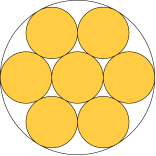
\includegraphics[width=0.2\textwidth]{Chapter-3/figs/CircleInCircle}
    \caption{Filter Rod Packing}
    \label{fig:CircleInCircle}
\end{figure}

\subsection{Raw Material Testing}
Tests on the raw cotton, and raw Cellulose Acetate provided were performed. In order to make each test consistent, the materials were weighted using clumped balls of $1.5$ grams. Five balls of equal weight were oriented into the machine, tested, and then averaged. This was done for the raw cotton balls and the raw Cellulose Acetate materials

\section{Impedance Tube Testing}

\subsection{Sample Preparation}
Each Sock sample was attached to an O-ring before it was loaded into the impedance tube testing section. Multiple layers of each Sock was created. 4 layers and 8 layers can be seen in the data shown in Chapter \ref{chap-four}.

\subsection{Setup}
Materials were configured for the 100mm and 29mm tubes. However, due to material limitations, all samples were tested in the 100mm tube. It is important to note that the smaller tube covers a broader range of frequencies, 500Hz to 6.3Hz, and hence dictates much better information about the overall performance of the material.

\subsection{Software}
Once the hardware and materials were properly configured, testing procedure continued on the attached laptop running PULSE software provided by Br�el \& Kj�r. Full details regarding the software can be found in Appendix \ref{append-B}.

\subsubsection{PULSE Software}
The PULSE software was used to collect data from the impedance tube system. The software was initialized, calibrated, and run in each test on every material. Each material was tested $5$ times and averaged to reduce hysteresis effects. The presented data in Chapter \ref{chap-four} is the averaged data. The data collected by the software was then exported into a spreadsheet file to be post-processed in MATLAB.

\subsubsection{MATLAB Software}
All data exported from PULSE was imported into MATLAB for analysis and graphical processing. The MATLAB scripts used for processing can be found in Appendix \ref{append-C}. Resultant graphs can be found in Chapter \ref{chap-four}.

\chapter{EXPERIMENTAL RESULTS}
\label{chap-four}

\section{Experimental Results}

This chapter presents the data from the experiment discussed in Chapter \ref{chap-three}.

\section{Base Data}
Readings in the impedance tube with no acoustic absorption material present are shown in this section.

% Absorption Coefficient - Empty
\begin{figure}[hbtp]
    \centering
    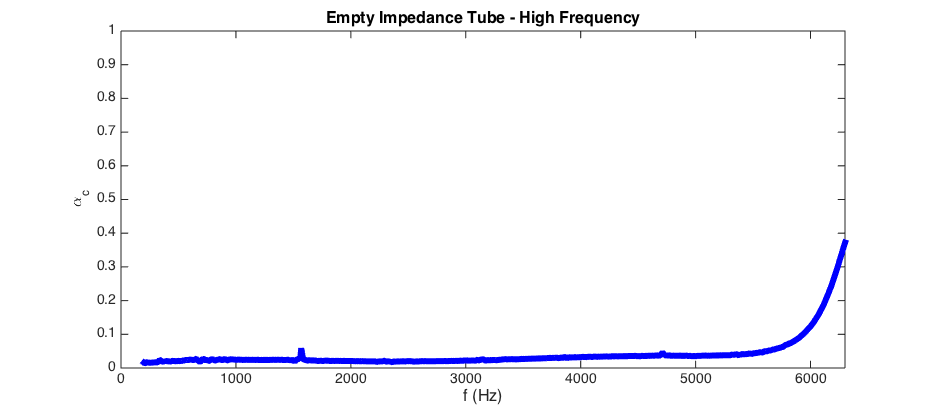
\includegraphics[width=1\textwidth]{Chapter-4/figs/Afigempty}
    \caption{Absorption Coefficient vs. Frequency - Empty Tube}
    \label{fig:Afigempty}
\end{figure}

Figure \ref{fig:Afigempty} shows the base values for absorption coefficient that the impedance tube system reads with no sample present.

% Absorption Coefficient - O Ring
\begin{figure}[hbtp]
    \centering
    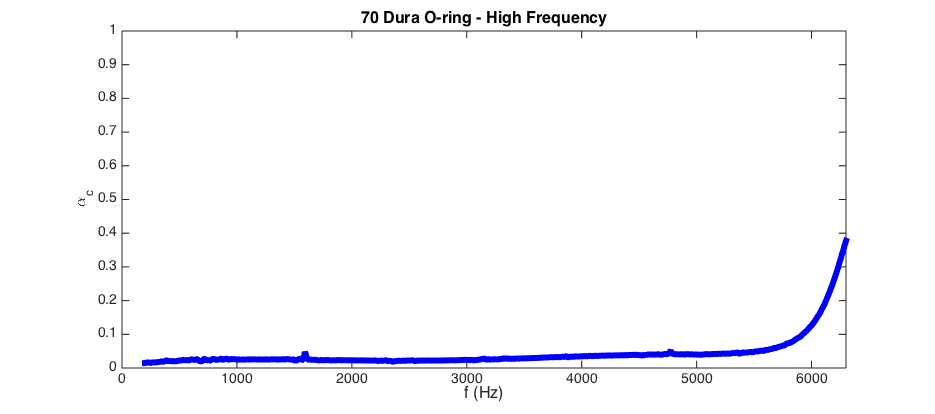
\includegraphics[width=1\textwidth]{Chapter-4/figs/AfigOring}
    \caption{Absorption Coefficient vs. Frequency - 70-Dura Oring}
    \label{fig:AfigOring}
\end{figure}
\clearpage
Figure \ref{fig:AfigOring} shows how adding the O-ring material has little influence in the data recorded by the system.

% Figures
\section{Commercial Materials}
Commercial material data is shown in this section.

\subsection{Foam Materials}
% Absorption Coefficient - BK Foam
\begin{figure}[hbtp]
    \centering
    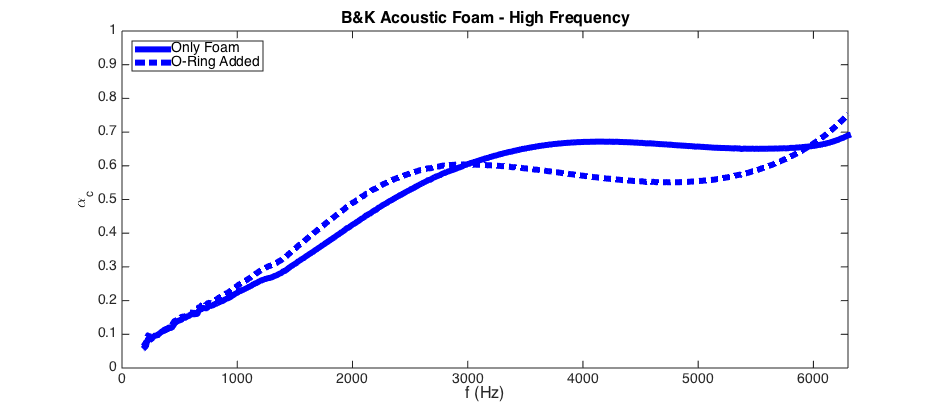
\includegraphics[width=1\textwidth]{Chapter-4/figs/AfigBKfoam}
    \caption{Absorption Coefficient vs. Frequency - B and K Foam}
    \label{fig:AfigBKfoam}
\end{figure}

% Absorption Coefficient - Auralex Foam
\begin{figure}[hbtp]
    \centering
    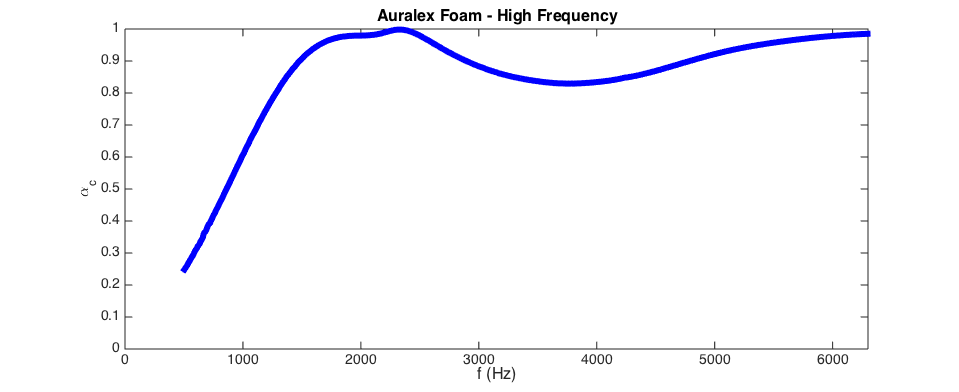
\includegraphics[width=1\textwidth]{Chapter-4/figs/AuralexFoam}
    \caption{Absorption Coefficient vs. Frequency - Auralex Foam}
    \label{fig:AuralexFoam}
\end{figure}
\clearpage

Figure \ref{fig:AfigBKfoam} and \ref{fig:AuralexFoam} show the results of the tests run for acoustic foams.

\subsection{Fiberglass}
% Absorption Coefficient - EX15-3 Fiberglass
\begin{figure}[hbtp]
    \centering
    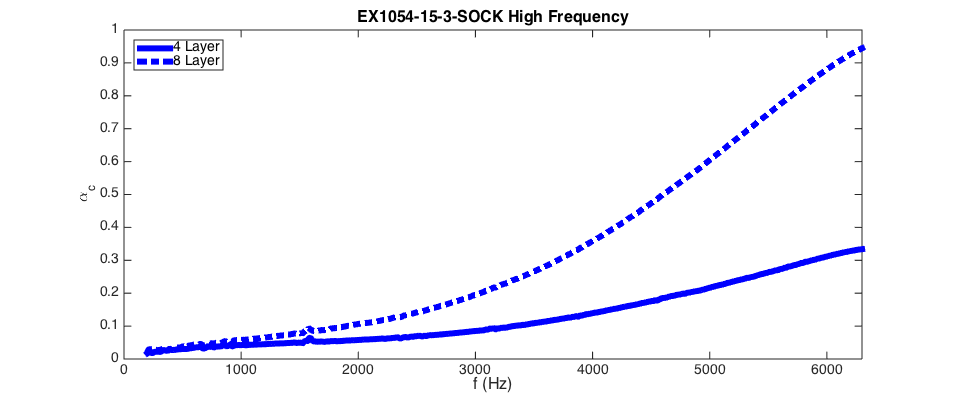
\includegraphics[width=1\textwidth]{Chapter-4/figs/AfigSOCK15-3}
    \caption{Absorption Coefficient vs. Frequency - EX1054-15-2 - Fiberglass}
    \label{fig:AfigSOCK15-3}
\end{figure}

% Absorption Coefficient - Raw Fiberglass (Thick - 2")
\begin{figure}[hbtp]
    \centering
    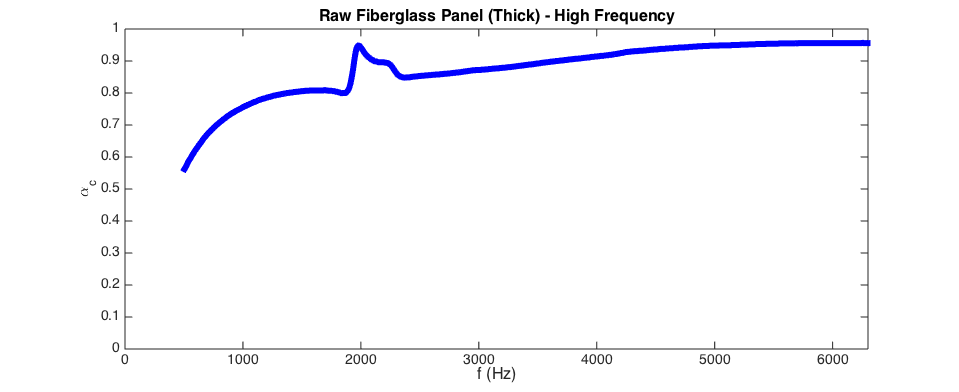
\includegraphics[width=1\textwidth]{Chapter-4/figs/RawFiberglassThick}
    \caption{Absorption Coefficient vs. Frequency - Raw Fiberglass (2" Thick)}
    \label{fig:RawFiberglassThick}
\end{figure}

% Absorption Coefficient - Raw Fiberglass (Thin - 1")
\begin{figure}[hbtp]
    \centering
    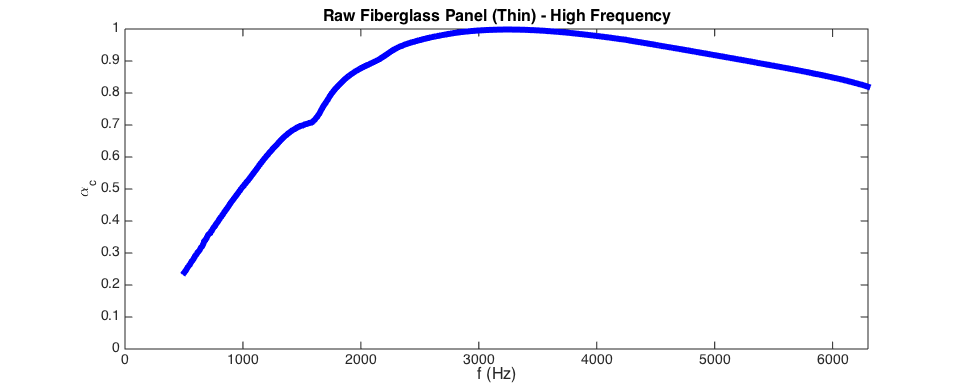
\includegraphics[width=1\textwidth]{Chapter-4/figs/RawFiberglassThin}
    \caption{Absorption Coefficient vs. Frequency - Raw Fiberglass (1" Thick)}
    \label{fig:RawFiberglassThin}
\end{figure}
\clearpage

Figure \ref{fig:AfigSOCK15-3} is a Sock type Fiberglass material, while figures \ref{fig:RawFiberglassThick} and \ref{fig:RawFiberglassThin} show a Fiberglass panel material in two thickness; 2" and 1" respectively.

\subsection{Polymer Materials}
% Absorption Coefficient - EX15-1 nylon
\begin{figure}[hbtp]
    \centering
    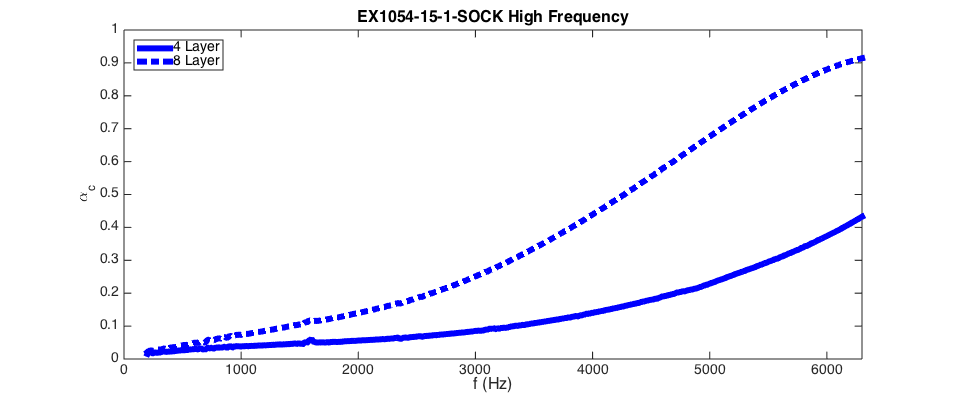
\includegraphics[width=1\textwidth]{Chapter-4/figs/AfigSOCK15-1}
    \caption{Absorption Coefficient vs. Frequency - EX1054-15-1 - Nylon}
    \label{fig:AfigSOCK15-1}
\end{figure}

% Absorption Coefficient - EX15-2 PET
\begin{figure}[hbtp]
    \centering
    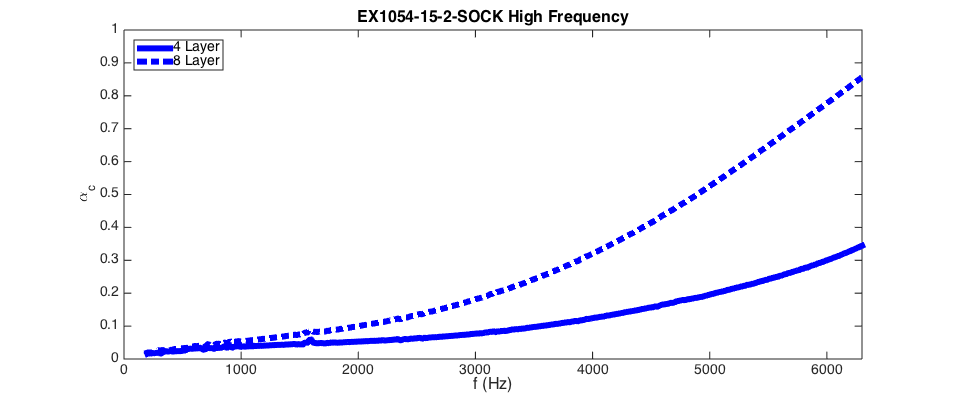
\includegraphics[width=1\textwidth]{Chapter-4/figs/AfigSOCK15-2}
    \caption{Absorption Coefficient vs. Frequency - EX1054-15-2 - PET}
    \label{fig:AfigSOCK15-2}
\end{figure}

% Absorption Coefficient - Auralex Cotton
\begin{figure}[hbtp]
    \centering
    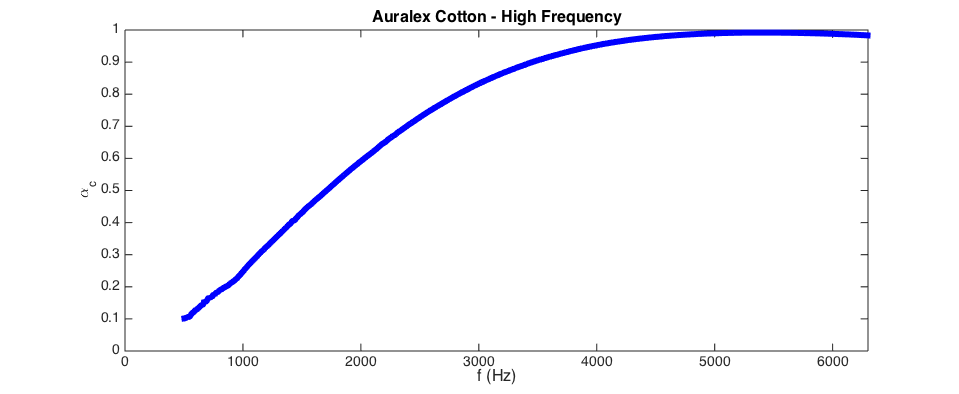
\includegraphics[width=1\textwidth]{Chapter-4/figs/AuralexCotton}
    \caption{Absorption Coefficient vs. Frequency - Auralex Cotton}
    \label{fig:AuralexCotton}
\end{figure}

% Absorption Coefficient - Auralex Compressed Polyester
\begin{figure}[hbtp]
    \centering
    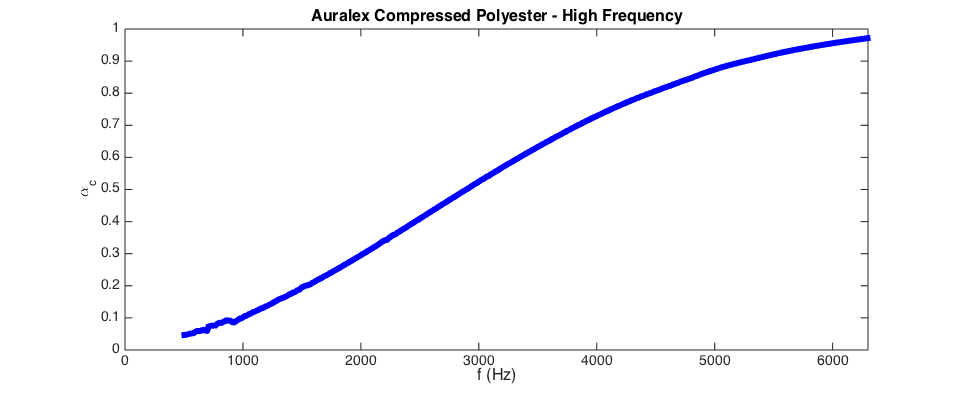
\includegraphics[width=1\textwidth]{Chapter-4/figs/AuralexCompPoly}
    \caption{Absorption Coefficient vs. Frequency - Auralex Compressed Polyester}
    \label{fig:AuralexCompPoly}
\end{figure}

Figures \ref{fig:AfigSOCK15-1}, and \ref{fig:AfigSOCK15-2} show sock materials of Nylon and PET respectively. Figure \ref{fig:AuralexCotton} shows compressed cotton from Auralex, and Figure \ref{fig:AuralexCompPoly} shows compressed polyester from Auralex.

\clearpage

\section{Cellulose Acetate Materials}
This section shows data for the Cellulose Acetate material tests.

% Absorption Coefficient - Raw Tow
\begin{figure}[hbtp]
    \centering
    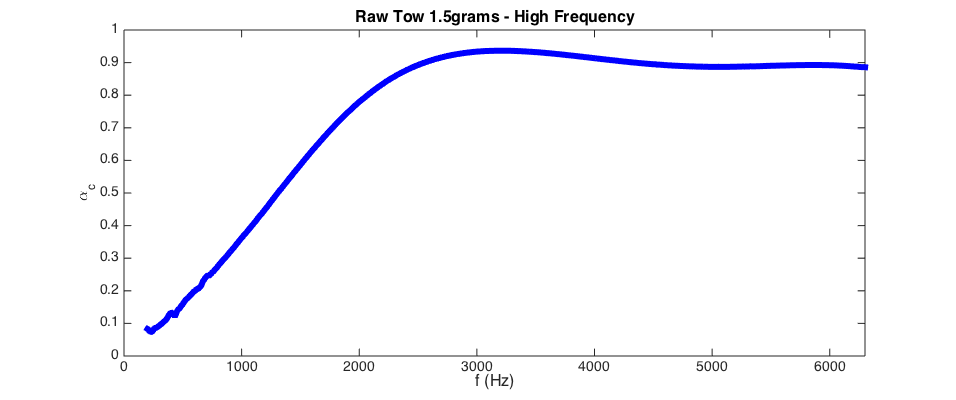
\includegraphics[width=1\textwidth]{Chapter-4/figs/Afigrawtow}
    \caption{Absorption Coefficient vs. Frequency - Raw Tow}
    \label{fig:Afigrawtow}
\end{figure}

Figure \ref{fig:Afigrawtow} shows the results from raw tow of $1.5$ grams.

\subsection{Sock Materials}
Cellulose Acetate Sock materials are presented below. They are divided into two sections for clarity: high and low denier respectively.
\clearpage

\subsubsection{High Denier Materials}
% Absorption Coefficient - EX8-2
\begin{figure}[hbtp]
    \centering
    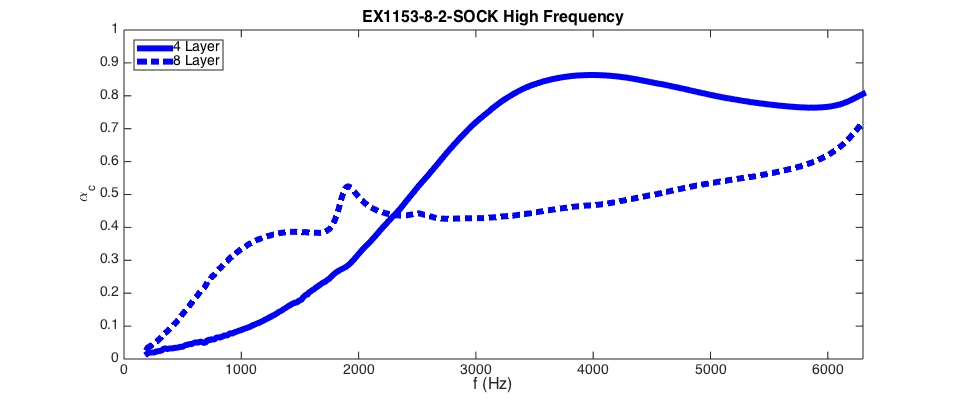
\includegraphics[width=1\textwidth]{Chapter-4/figs/AfigSOCK8-2}
    \caption{Absorption Coefficient vs. Frequency - EX1154-8-2}
    \label{fig:AfigSOCK8-2}
\end{figure}

% Absorption Coefficient - EX9-5
\begin{figure}[hbtp]
    \centering
    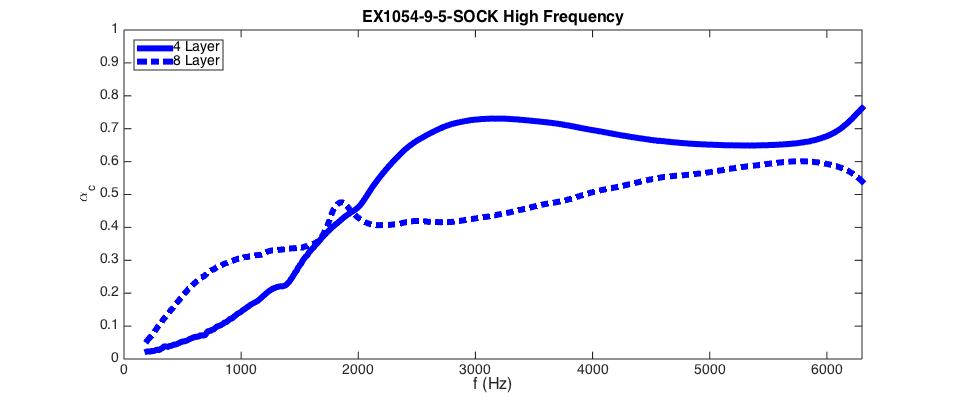
\includegraphics[width=1\textwidth]{Chapter-4/figs/AfigSOCK9-5}
    \caption{Absorption Coefficient vs. Frequency - EX1054-9-5}
    \label{fig:AfigSOCK9-5}
\end{figure}

% Absorption Coefficient - EX9-6
\begin{figure}[hbtp]
    \centering
    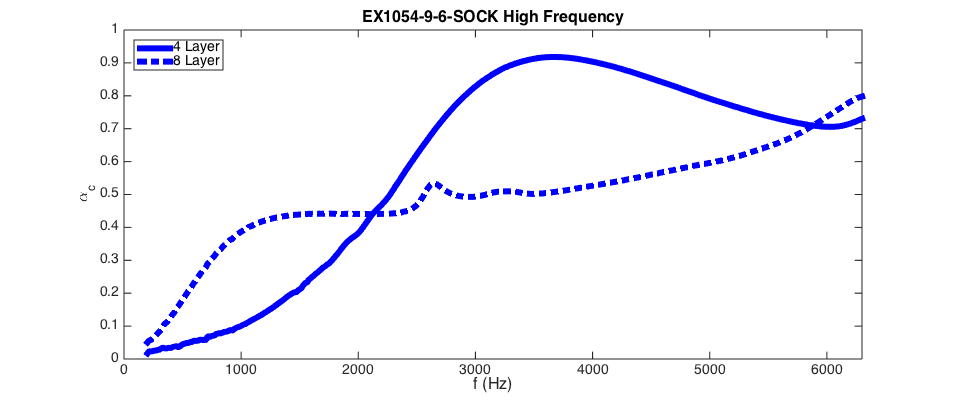
\includegraphics[width=1\textwidth]{Chapter-4/figs/AfigSOCK9-6}
    \caption{Absorption Coefficient vs. Frequency - EX1054-9-6}
    \label{fig:AfigSOCK9-6}
\end{figure}

% Absorption Coefficient - EX18-3
\begin{figure}[hbtp]
    \centering
    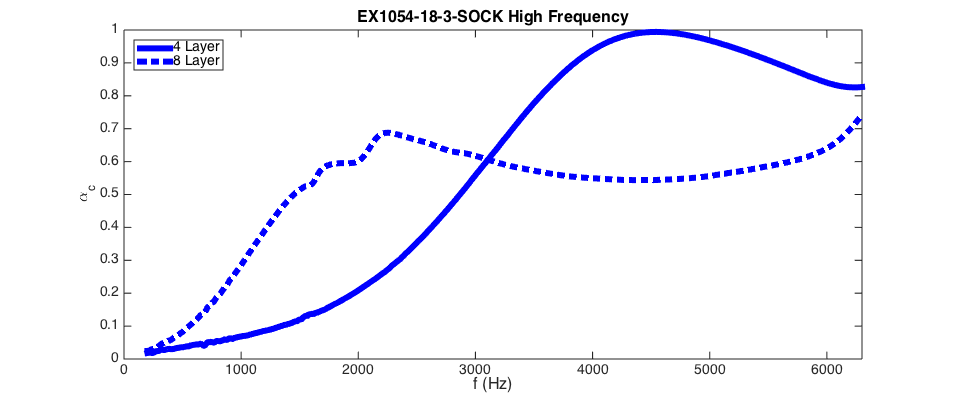
\includegraphics[width=1\textwidth]{Chapter-4/figs/AfigSOCK18-3}
    \caption{Absorption Coefficient vs. Frequency - EX1054-18-3}
    \label{fig:AfigSOCK18-3}
\end{figure}

% Absorption Coefficient - EX18-4
\begin{figure}[hbtp]
    \centering
    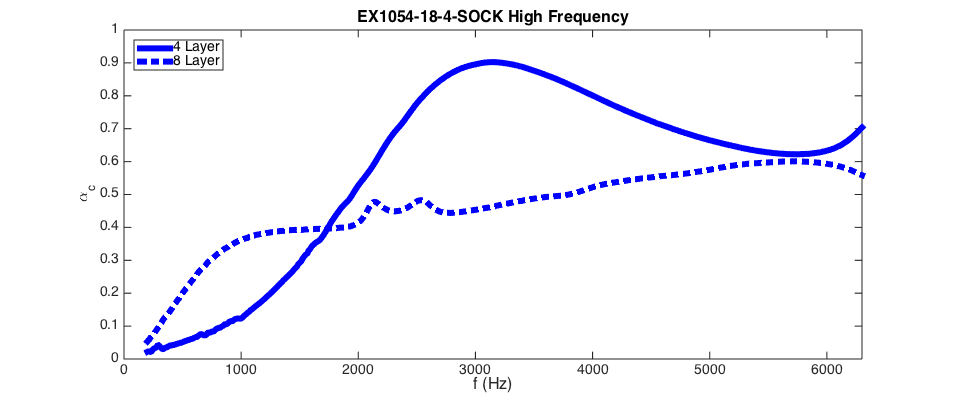
\includegraphics[width=1\textwidth]{Chapter-4/figs/AfigSOCK18-4}
    \caption{Absorption Coefficient vs. Frequency - EX1054-18-4}
    \label{fig:AfigSOCK18-4}
\end{figure}
\clearpage

\subsubsection{Low Denier Materials}

% Absorption Coefficient - EX9-1
\begin{figure}[hbtp]
    \centering
    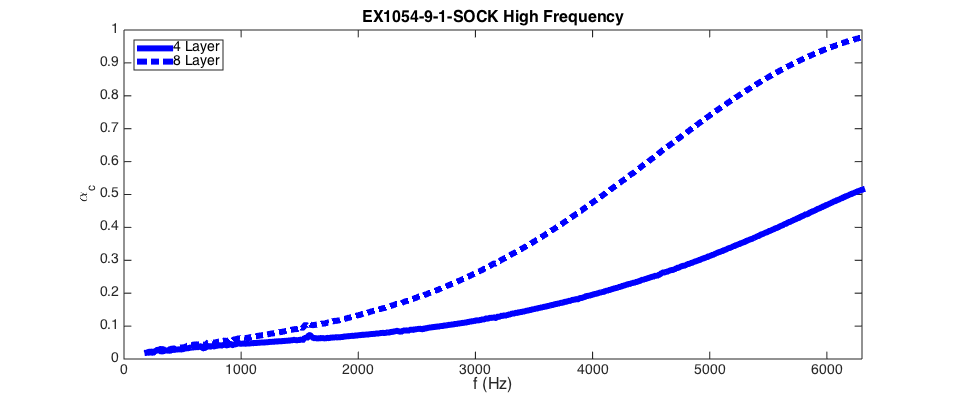
\includegraphics[width=1\textwidth]{Chapter-4/figs/AfigSOCK9-1}
    \caption{Absorption Coefficient vs. Frequency - EX1054-9-1}
    \label{fig:AfigSOCK9-1}
\end{figure}

% Absorption Coefficient - EX9-3
\begin{figure}[hbtp]
    \centering
    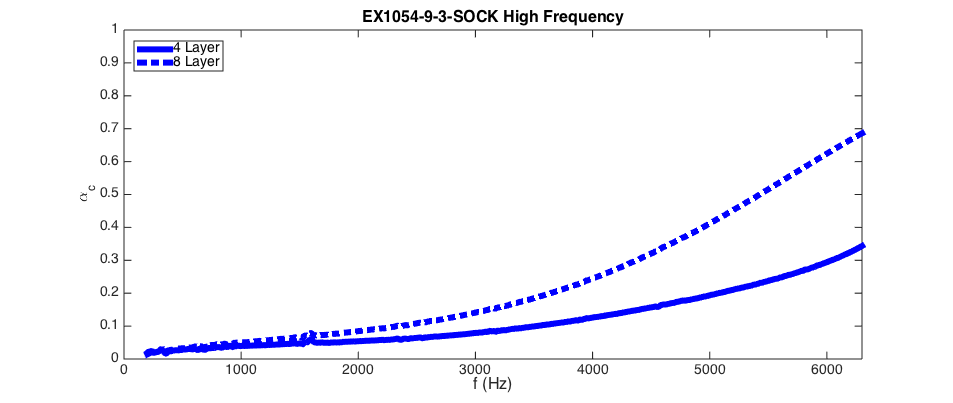
\includegraphics[width=1\textwidth]{Chapter-4/figs/AfigSOCK9-3}
    \caption{Absorption Coefficient vs. Frequency - EX1054-9-3}
    \label{fig:AfigSOCK9-3}
\end{figure}

% Absorption Coefficient - EX9-8
\begin{figure}[hbtp]
    \centering
    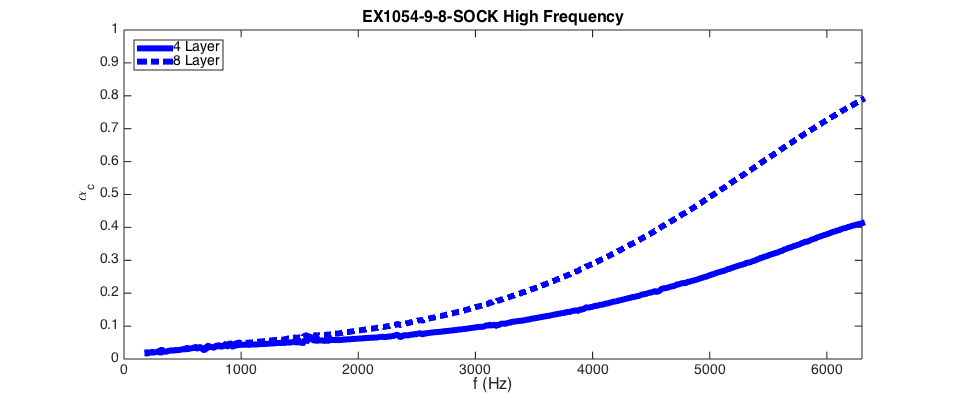
\includegraphics[width=1\textwidth]{Chapter-4/figs/AfigSOCK9-8}
    \caption{Absorption Coefficient vs. Frequency - EX1054-9-8}
    \label{fig:AfigSOCK9-8}
\end{figure}

% Absorption Coefficient - EX9-9
\begin{figure}[hbtp]
    \centering
    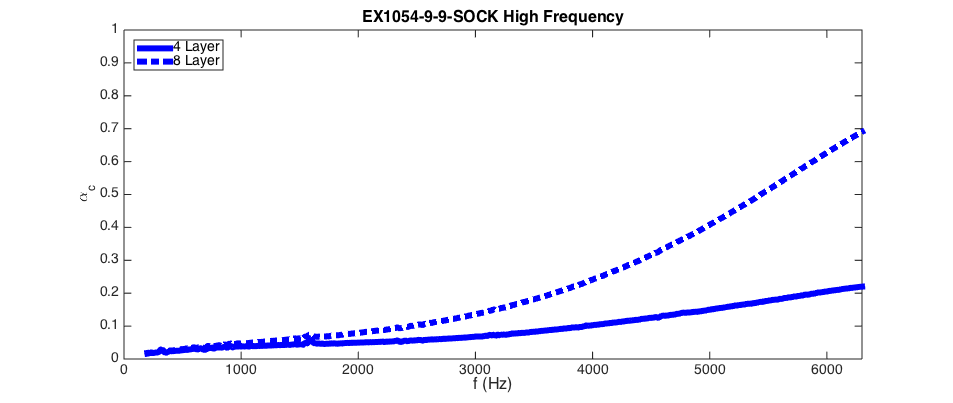
\includegraphics[width=1\textwidth]{Chapter-4/figs/AfigSOCK9-9}
    \caption{Absorption Coefficient vs. Frequency - EX1054-9-9}
    \label{fig:AfigSOCK9-9}
\end{figure}

% Absorption Coefficient - EX18-1
\begin{figure}[hbtp]
    \centering
    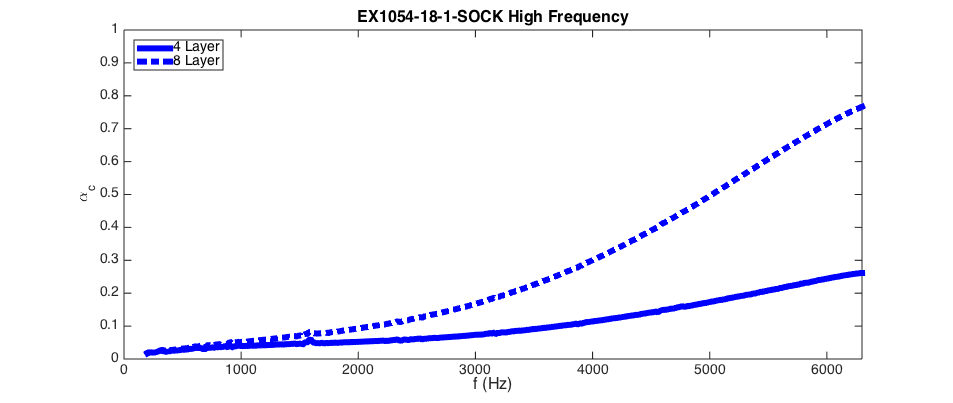
\includegraphics[width=1\textwidth]{Chapter-4/figs/AfigSOCK18-1}
    \caption{Absorption Coefficient vs. Frequency - EX1054-18-1}
    \label{fig:AfigSOCK18-1}
\end{figure}

% Absorption Coefficient - EX18-2
\begin{figure}[hbtp]
    \centering
    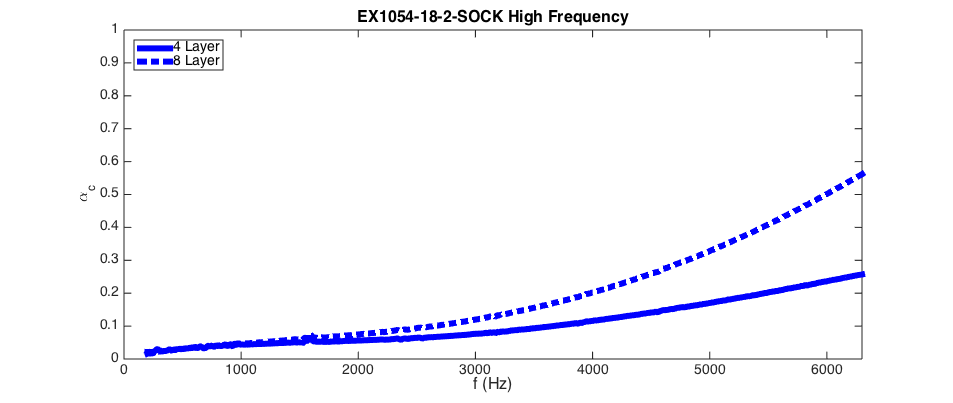
\includegraphics[width=1\textwidth]{Chapter-4/figs/AfigSOCK18-2}
    \caption{Absorption Coefficient vs. Frequency - EX1054-18-2}
    \label{fig:AfigSOCK18-2}
\end{figure}
\clearpage




\subsection{Filter Rod Materials}
Filter Rod test data is presented below.

% Absorption Coefficient - Filter Rod White
\begin{figure}[hbtp]
    \centering
    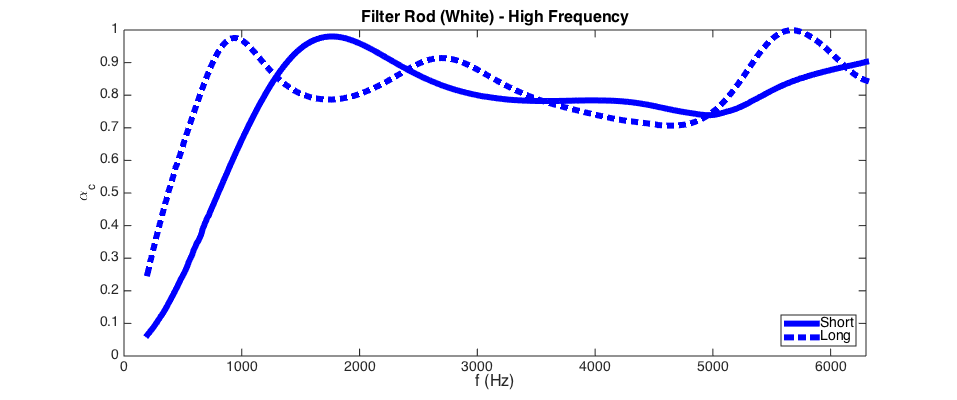
\includegraphics[width=1\textwidth]{Chapter-4/figs/Afigfilterrodwhite}
    \caption{Absorption Coefficient vs. Frequency - White Filter Rod}
    \label{fig:Afigfilterrodwhite}
\end{figure}

% Absorption Coefficient - Filter Rod White no paper
\begin{figure}[hbtp]
    \centering
    \includegraphics[width=1\textwidth]{Chapter-4/figs/Afigfilterrodwhitenopaper}
    \caption{Absorption Coefficient vs. Frequency - White Filter Rod (no paper)}
    \label{fig:Afigfilterrodwhitenopaper}
\end{figure}

% Absorption Coefficient - Filter Rod Black
\begin{figure}[hbtp]
    \centering
    \includegraphics[width=1\textwidth]{Chapter-4/figs/Afigfilterrodblack}
    \caption{Absorption Coefficient vs. Frequency - Black Filter Rod}
    \label{fig:Afigfilterrodblack}
\end{figure}

% Absorption Coefficient - Filter Rod Black no paper
\begin{figure}[hbtp]
    \centering
    \includegraphics[width=1\textwidth]{Chapter-4/figs/Afigfilterrodblacknopaper}
    \caption{Absorption Coefficient vs. Frequency - Black Filter Rod (no paper)}
    \label{fig:Afigfilterrodblacknopaper}
\end{figure}
\clearpage

\section{Comparing Materials}
After all data has been recorded, trends between data sets start to arise. This section overlays data sets to show similar data. 

\subsection{High Denier vs. Low Denier Mix}
This section compares a sample of relatively high denier with a sample of relatively low denier of equal mass.

% Absorption Coefficient - SOCK 18-3 vs. 9-1
\begin{figure}[hbtp]
    \centering
    \includegraphics[width=1\textwidth]{Chapter-4/figs/AfigSOCK18-3compareSOCK9-1}
    \caption{Absorption Coefficient vs. Frequency - SOCK18-3 vs. SOCK9-1}
    \label{fig:AfigSOCK18-3compareSOCK9-1}
\end{figure}

% Absorption Coefficient - SOCK 18-3 vs. 9-9
\begin{figure}[hbtp]
    \centering
    \includegraphics[width=1\textwidth]{Chapter-4/figs/AfigSOCK18-3compareSOCK9-9}
    \caption{Absorption Coefficient vs. Frequency - SOCK18-3 vs. SOCK9-9}
    \label{fig:AfigSOCK18-3compareSOCK9-9}
\end{figure}

% Absorption Coefficient - SOCK 18-4 vs. 9-3
\begin{figure}[hbtp]
    \centering
    \includegraphics[width=1\textwidth]{Chapter-4/figs/AfigSOCK18-4compareSOCK9-3}
    \caption{Absorption Coefficient vs. Frequency - SOCK18-4 vs. SOCK9-3}
    \label{fig:AfigSOCK18-4compareSOCK9-3}
\end{figure}
\clearpage

\subsection{All Sock Data}
This section shows all the Sock data compiled.

% Absorption Coefficient - all compared SOCKS
\begin{figure}[hbtp]
    \centering
    \includegraphics[width=1\textwidth]{Chapter-4/figs/AfigSOCKScompared}
    \caption{Absorption Coefficient vs. Frequency - All Compared SOCKS}
    \label{fig:AfigSOCKScompared}
\end{figure}
\clearpage

\subsection{Cellulose Acetate Sock Compared with Fiberglass}
% Absorption Coefficient - all compared SOCKS w/ Fiberglass
\begin{figure}[hbtp]
    \centering
    \includegraphics[width=1\textwidth]{Chapter-4/figs/AfigSOCKScomparefiberglass}
    \caption{Absorption Coefficient vs. Frequency - All Compared SOCKS with Fiberglass}
    \label{fig:AfigSOCKScomparefiberglass}
\end{figure}
\clearpage

\subsection{Filter Rods}
This section shows the filter rods as compared with Raw tow of equal mass.
% Absorption Coefficient - Raw Tow vs. Filter Rods 1.5 grams
\begin{figure}[hbtp]
    \centering
    \includegraphics[width=1\textwidth]{Chapter-4/figs/Afigfilterrodscomparerawtow}
    \caption{Absorption Coefficient vs. Frequency - Raw Tow vs. Filter Rods}
    \label{fig:Afigfilterrodscomparerawtow}
\end{figure}

% Absorption Coefficient - Raw Tow vs. Filter Rods vs. Cotton
\begin{figure}[hbtp]
    \centering
    \includegraphics[width=1\textwidth]{Chapter-4/figs/Afigfilterrodscomparerawtowcomparecotton}
    \caption{Absorption Coefficient vs. Frequency - Raw Tow vs. Filter Rods vs. Cotton}
    \label{fig:Afigfilterrodscomparerawtowcomparecotton}
\end{figure}
\clearpage

\subsection{Raw Tow}
Raw Tow was analyzed with respect to Cotton of equal mass of $1.5$ grams.
% Absorption Coefficient - Raw Tow vs. Cotton 1.5 grams
\begin{figure}[hbtp]
    \centering
    \includegraphics[width=1\textwidth]{Chapter-4/figs/Afigrawtowcomparecotton}
    \caption{Absorption Coefficient vs. Frequency - Raw Tow vs. Cotton 1.5 grams}
    \label{fig:Afigrawtowcomparecotton}
\end{figure}

\chapter{RESULTS DISCUSSION}
\label{chap-five}

\section*{Results Discussion}

This chapter will discuss the results presented in Chapter \ref{chap-four}.

\section{Material Consideration}

Various types of materials were used in the tests in the experiments.

\subsection{Commercial Material Categories}
The commercial tests were run on various samples. The samples were provided by Auralex Acoustics, and Eastman Chemical Company. There were 4 categories of materials tested. Various materials were tested within each of the $4$ categories. They were as follows:
\begin{enumerate}
	\item Sock Materials
		\begin{enumerate}
			\item Fiberglass Sock
			\item PET Sock
			\item Nylon Sock
		\end{enumerate}
	\item Raw Material Type
		\begin{enumerate}
			\item Raw Cotton Balls
			\item Auralex Compressed Cotton
		\end{enumerate}
	\item Acoustic Foam Type
		\begin{enumerate}
			\item Br�el \& Kj�r Foam
			\item Auralex Acoustics Foam
		\end{enumerate}
	\item Acoustic Panneling Type
		\begin{enumerate}
			\item Owens Corning Fiberglass Panel
			\item	Auralex Compressed Polyester Panel
		\end{enumerate}
\end{enumerate}
These categories represent each of the major types of absorption materials presently used today.

\subsection{Cellulose Acetate Material Categories}
The tests on the Cellulose Acetate can be broken down into 3 categories.
\begin{enumerate}
	\item Sock Materials
	\item Filter Rods
	\item Raw Tow
\end{enumerate}
These categories represent various types of manufacturing Cellulose Acetate in order to adequately analyze its utility as an absorption material.

\subsection{Matching Similar Commercial Materials to Cellulose Acetate}
To appropriately match the Cellulose Acetate material types to commercial materials, a wide range of materials were tested.\\
\indent The Sock materials provided much insight into Cellulose Acetates acoustic performance characteristics, and logically, were paired for comparison with the commercial sock materials. All of the Sock tests were performed using 4 and 8 layers of material to show a relationship between the thickness of absorption material present in the data.\\
\indent The Cellulose Acetate Filter Rods were compared against a few different materials, since there was not any directly similar material available. The rods were compared against raw cotton, and raw tow.\\
\indent The acoustic foams and paneling are commonly used commercially and were tested for data comparison.\\

\section{Considering Frequency Band}

In testing the materials two sizes of the impedance tubes were used. The large 100mm portion covered $50 \text{Hz}$ to $1600 \text{Hz}$ while the smaller 29mm portion covered $500 \text{Hz}$ to $6300 \text{Hz}$. It should be noted that for a theoretical impedance tube the working frequency range can span across a wide range of frequencies as noted in standards ISO-10534-2 \cite{ISO1998}, ASTM E1050-12 \cite{ASTM1990} and ASTM E2611-09 \cite{ASTM2011}. Calculations shown in Table \ref{tab:workingfreq} suggest that a larger frequency band may have been acceptable with this testing equipment. However the suggested frequencies by the tube's manufacturer were used.\\
\indent After collecting data on all samples which enough material was available for, it was determined that the smaller 29mm tube provided much better data than the larger tube which focused on lower frequencies. The broader range of data collected in the 29mm tube proved much more useful in showing the response of the materials. For this reason, a majority of the lower frequency data was thrown out. The presented data is that from the 29mm tube, e.g. $500 \text{Hz}$ to $6300 \text{Hz}$. Generally for human comfort level, the range between $2000 \text{Hz}$ and $4000 \text{Hz}$ is considered.

\section{Measurement Errors}
Each of these tests run in the Br�el \& Kj�r Impedance tube experienced small amounts of error due to imperfect materials and imperfect testing techniques. The performer of the experiment aimed to minimize these effects.

\subsection{Mechanical Resonance}
Mechanical resonance is caused when the skeletal structure of a porous material hits a frequency that matches the skeletal structure's natural frequency of vibration. Certain commercial and Cellulose materials present mechanical resonance which results in increased absorption within a narrow frequency range surrounding the natural frequency of vibration of the skeletal structure.

\subsubsection{Sock Materials}
Some of the materials showed abrupt peaks in their Absorption across the frequency spectrum. In particular, Figures \ref{fig:AuralexFoam}, \ref{fig:RawFiberglassThick}, \ref{fig:AfigSOCK8-2}, \ref{fig:AfigSOCK9-5}, \ref{fig:AfigSOCK9-6}, \ref{fig:AfigSOCK18-3}, \ref{fig:AfigSOCK18-4} showed a spike in absorption coefficient around $2000 \text{Hz}$. This is because these materials have a higher denier and thus were stiffer than the other samples. This resulted in the skeletal structure of the material hitting its resonant frequency. When the mode of the resonant frequency is excited, a small frequency band surrounding the center resonant frequency experience a higher amount of absorption.

\subsubsection{Filter Rod Materials}
The tests on the filter rod materials also presented some peaks in the lower frequency ranges due to the stiffer material hitting its resonance frequency. Figures \ref{fig:Afigfilterrodwhite}, and \ref{fig:Afigfilterrodblack} show a spike in the $1000 \text{Hz}$ to $2000 \text{Hz}$ range for samples with paper attached. The same samples tested without paper in figures \ref{fig:Afigfilterrodwhitenopaper}, and \ref{fig:Afigfilterrodblacknopaper} show a mechanical resonance spike in a similar range. This is more difficult to see due to the higher frequencies showing slightly different values.

\subsection{O-ring Considerations}
The testing set up on the Sock type materials needs to be considered. In order to allow the Sock materials to properly lay in the testing region, the samples were stapled to a rubber O-ring material. This O-ring provided some noise in the measurement. Tests were run in the Impedance Tube using only the O-ring. It can be seen in Figure \ref{fig:AfigOring} that the O-ring provided some additionally read absorption in the high frequencies. However, this can be ignored when it is compared with the measured reading in the empty tube in Figure \ref{fig:Afigempty}. 

\subsection{Air Gaps}
In an impedance tube measurement system, any present air gaps result in recording a higher value of absorption coefficient. This results in data that is not true to the materials absorption characteristics. This means that air gaps may have resulted in some data collected by the analysis system being inaccurate. This is an inevitability of an imperfect process of creating test samples as limited by the resources available.

\subsubsection{Filter Rod Materials}
The filter rod tests performed well as can be seen in the papered tests figures \ref{fig:Afigfilterrodwhite}, \ref{fig:Afigfilterrodblack} and the paperless tests figures \ref{fig:Afigfilterrodwhitenopaper} and \ref{fig:Afigfilterrodblacknopaper}. However, each of these tests had significant air gaps present. In order to properly input the filter rods into the impedance tube, the filter rods had to be packed in the diameter of the rubber O-ring for support. The air gaps are clearly seen in Figure \ref{fig:CircleInCircle}, which shows yellow filter rods, and the white air gaps.\\

\begin{figure}[hbtp]
    \centering
    \includegraphics[width=0.3\textwidth]{Chapter-5/figs/CircleInCircle}
    \caption{Air Gap in Filter Rod Test - Yellow is Filter Rods, White is Air Gap }%\cite{Circle}}
    \label{fig:CircleInCircle}
\end{figure}

This percentage of air gap means that the filter rods data is artificially higher than the true value should be. In order to correct this error, filter rods of the exact size of the impedance tube (29mm) would need to be manufactured and tested to eliminate the air gap error. However, due to resources available, this test was unable to be performed.

\section{Health Impact}
A tremendous benefit to Cellulose Acetate Tow as an absorption material is its biocompatibility. Fibrous materials generally have their strongest absorption effects at higher frequencies, while lower frequencies have lower absorption effects. This is true for current industry standards. However, Cellulose Acetate provides similar performance characteristics to that of fiberglass. This allows Cellulose Acetate to be considered for use in environments when fiberglass would be unacceptable. An example of this would be an environment requiring no health risks, however, suffers from large durations and magnitudes of noise. An applicable environment could be medical in nature, such as a hospital emergency unit would require. The ability for designers to control the acoustic level in such an environment would be greatly benefit the patients and employees.

\section{Cost}
Results show Cellulose Acetate is a good alternative to commercial absorption materials. However, this must be looked at in regards to cost of the material. Fiberglass is a popular material in the absorption field. Part of the reason it is so popular is it is extremely cheap. Cellulose Acetate is more difficult to manufacture and consequently more expensive. However this premium comes with the added benefit of biofriendliness.\\
\indent Within the CA samples, there are some clear differences. The best overall performing was the Sock sample label 9-5 Figure \ref{fig:AfigSOCK9-5}, which had a Total Denier of 1576, a DPF of 2, 788 Filaments, and a Y cross section. However, this material is more difficult to work with than some of the relatively lower denier CA samples. The larger fiber size of the High Denier samples can be messy to work with. After working with one of these materials, lots of smaller particles get everywhere, which depending on the situation would not be ideal. This logistical cost is much higher than that of the lower denier finer knit fibers. These are easy to work with and do not get as messy as the larger ones. Pending on the situation, a higher denier or lower denier with many layer type of Tow would be needed.\\
\indent The CA sample labeled 9-3 Figure \ref{fig:AfigSOCK9-3}, which has a Total Denier of 150, a DPF of 6, 25 filaments, and a 8 Leg cross section, showed poor absorption performance, but has a better logistical cost. Since it has fine fibers, it is much easier to work with and depending on the scenario could be the ideal choice. The performance can be increased by using multiple layers.

\chapter{CONCLUSION}
\label{chap-six}

\section*{Conclusion}
This chapter provides a conclusion to the work discussed in previous chapters.

\section{Summary}
This paper presents an investigation into Cellulose Acetate Tow (CA) as an acoustic absorption material. Research in this field is of growing interest, as noise pollution is considered to be a major health concern. Samples of CA were tested in various manufactured configurations in a Br�el \& Kj�r Impedance Tube Type 4206A. A variety of commercial absorption materials were also tested and are compared to the acoustic performance characteristics of Cellulose Acetate Tow.\\
\indent To appropriately analyze the problem, necessary mathematical background is developed and a review of current literature in the theory regarding acoustic absorption has been reviewed in Chapter \ref{chap-two}. Key parameters for the fibers, chemistry, and poroelasticity have been presented and discussed. Empirical models of porous materials and measurement techniques are also discussed. Finally, the impedance tube method definition as used by the experimental set-up is also covered.\\
\indent Chapter \ref{chap-three} covers the experiment design and configuration used in the investigation. A complete list of materials is presented. Considerations regarding the testing preparation are also discussed. The impedance tube testing process is given. A detailed step-by-step outline for the equipment can be found in Appendix \ref{append-B}.\\
\indent Experimental results are presented in Chapter \ref{chap-four} for each specimen. Results show data from $500 \text{Hz}$ to $6300 \text{Hz}$, however, tests on lower frequencies were also performed. The low frequency information have been omitted in order to show the most relevant data. Implications of the experimental data shown in Chapter \ref{chap-four} are discussed in detail in Chapter \ref{chap-five}. After the analysis of the data, the appropriate concerns and findings have been discussed.\\
\indent Similar experiments designed for measuring acoustic properties of biologically friendly materials have been performed in literature \cite{Ersoy2009} and \cite{Wassilieff1996}. This paper aims to provide a new material in the field of biologically friendly porous media used for acoustic absorption. As can be see in Chapters \ref{chap-four} and \ref{chap-five}, Cellulose Acetate shows promise as an effective alternative to current materials.\\
\indent While it can be seen in Figure \ref{fig:AfigSOCKScomparefiberglass} that some CA materials perform slightly better or slightly worse than fiberglass, it should be noted that cost of the materials is important. This is both in financial and logistical cost.The samples with the best performance, the high denier, are more difficult to work with and thus have a higher logistical cost than the lower denier lesser performing materials. The issue with the higher denier materials is they are messy to work with and this is not suitable for all environments. A finer material is much easier to work with and while less performing, potentially more suitable.

\subsection{Future Work}
This work provides background for future research in this subject. Due to the complex nature of porous media absorption problems, the key poroelastic parameters needed for performance optimization are difficult to identify. Possible future work includes investigation in the optimal performance of the material. This can be done by considering a study on the ratio of filler material in the Cellulose Acetate. This was considered outside of the scope of the present project. Another potential research topic is investigating the accuracy of empirical methods discussed in Chapter \ref{chap-two} by comparing results to experimental data presented in this paper.

%\restoregeometry
%%---------------------------------------------------------------------------%%
%%  Bibliography 

%%  You can use the bibitem list.
%\bibliographystyle{unsrt}
%\begin{%thebibliography}{99}
%\bibitem{cb02}
%Casella, G. and Berger, R.L. (2002)
%\newblock {\it Statistical Inference, Second Edition.}
%Duxbury Press, Belmont, CA.
%
%\bibitem{t06}
%Tsiatis, A.A. (2006)
%\newblock {\it Semiparametric Theory and Missing Data.}
%Springer, New York.
%
%\end{thebibliography}

%% or use BibTeX
%\bibliography{Ortiz-thesis}{}
%\bibliographystyle{plain}
%\nociterec{*}

%\bibliographystyle{plainnat}%plainnat is necessary to enable the use of citet. Natbib style file.
%\bibliography{Ortiz-thesis2}
%\ensureoddstart
\begin{spacing}{1}
 \setlength\bibitemsep{11pt} %22pt = 2*11pt, where fontsize is 11pt
 \addcontentsline{toc}{chapter}{{\uppercase{\bibname}}} %\textorpdfstring and \uppercase needed due to hyperref package http://www.latex-community.org/forum/viewtopic.php?f=44&t=16601
 %\vspace{-0.5in}
\titleformat{\chapter}[display]{\bf\filcenter
}{\chaptertitlename\ \thechapter}{11pt}{\bf\filcenter}
\titlespacing*{\chapter}{0pt}{-0.5in-9pt}{22pt}

\printbibliography[heading=myheading]
\end{spacing}
%\bibliographystyle{apalike}

%%---------------------------------------------------------------------------%%
% Appendices
%\ensureoddstart
\restoregeometry
\appendix
\newgeometry{margin=1in,lmargin=1.25in,footskip=\chapterfootskip, includehead, includefoot}
\chapter{NOMENCLATURE}
\label{append-A}

\section*{Nomenclature}
This appendix provides a list of variables used throughout the paper.

% Page 1
\begin{table}
    \caption{Nomenclature pt. 1}
    \label{tab:nomenclature1}
    \begin{center}
    \begin{tabular}{lcl}
    \toprule
    Variable & \ldots{} & Definition\\
    \midrule
    $B_e$ & \ldots{} & Effective Bulk Modulus\\
    $c$ & \ldots{} & Speed of Sound\\
    $c_0$ & \ldots{} & Speed of Sound at 1 atm\\
    $C_i$ & \ldots{} & Pressure Wave Incident Coefficient\\
    $C_r \text{ or } R$ & \ldots{} & Pressure Wave Reflection Coefficient\\
    $C_P$ & \ldots{} & Heat Capacity at Constant Pressure\\ 
    $C_V$ & \ldots{} & Heat Capacity at Constant Volume\\
    $DPF$ & \ldots{} & Denier per Filament\\
    $E$ & \ldots{} & Youngs Modulus; Normalized Frequency Parameter (Mechel-V�r Model)\\
    $E^{*}$ & \ldots{} & Complex Modulus\\
    $E'$ & \ldots{} & Storage Modulus\\
    $E''$ & \ldots{} & Loss Modulus\\
    $f$ & \ldots{} & Frequency\\
    $f_l$ & \ldots{} & Lower Working Frequency\\
    $f_u$ & \ldots{} & Upper Working Frequency\\
    $F_r$ & \ldots{} & Viscous Frictional Force\\
    $G$ & \ldots{} & Shear Modulus\\
    $H$ & \ldots{} & Frequency Response Function\\
    $H_C$ & \ldots{} & Calibration Factor\\
    $H_i$ & \ldots{} & Incident Frequency Response Function\\
    $H_r$ & \ldots{} & Reflection Frequency Response Function\\
    $I$ & \ldots{} & Acoustic Intensity\\
    $I_ref$ & \ldots{} & ReferenceAcoustic Intensity\\
    $IL$ & \ldots{} & Intensity Level\\
    $j$ & \ldots{} & Complex Number $\sqrt{-1}$\\
    $k$ & \ldots{} & Wave Number\\ 
    $K$ & \ldots{} & Compressibility Modulus\\ 
    $p$ & \ldots{} & Acoustic Pressure\\
    $P$ & \ldots{} & Peak Acoustic Pressure\\    
    $P_e$ & \ldots{} & Effective Acoustic Pressure\\
    $P_r$ & \ldots{} & Prandtl Number\\
    $P_ref$ & \ldots{} & Reference Acoustic Pressure\\
    $r$ & \ldots{} & Specific Gas Constant; Specific Acoustic Resistance\\
    $R$ & \ldots{} & Complex Reflection Coefficient\\
    $\mathbf{R}$ & \ldots{} & Normal Incidence Reflection Coefficient\\
    $R_m$ & \ldots{} & Mechanical Resistance\\
    \bottomrule
    \end{tabular}
    \end{center}
\end{table}

% Page 2
\begin{table}
    \caption{Nomenclature pt. 2}
    \label{tab:nomenclature2}
    \begin{center}
    \begin{tabular}{lcl}
    \toprule
    Variable & \ldots{} & Definition\\
    \midrule
    $S$ & \ldots{} & Surface Area\\
    $SPL$ & \ldots{} & Sound Pressure Level\\
    $T$ & \ldots{} & Period\\
    $T_g$ & \ldots{} & Glass Transition Temperature\\
    $T_K$ & \ldots{} & Absolute Temperature (Kelvin)\\
    $\overrightarrow{u}$ & \ldots & Particle Velocity\\
    $V_0$ & \ldots{} & Residual Volume in sample chamber\\
    $V_a$ & \ldots{} & Total Air Filled Volume\\
    $V_t$ & \ldots{} & Total Volume\\
    $x$ & \ldots{} & Specific Acoustic Reactance\\
    $X$ & \ldots{} & Frequency Parameter (Delany and Bazley Model)\\
    $X_m$ & \ldots{} & Mechanical Reactance\\
    $Z$ & \ldots{} & Impedance\\
    $z$ & \ldots{} & Specific Acoustic Impedance\\
    $Z_n$ & \ldots{} & Normalized Impedance\\
    $Z_m$ & \ldots{} & Mechanical Impedance\\
    $\alpha$ & \ldots{} & Absorption Coefficient\\
    $\alpha_c$ & \ldots{} & Characteristic Absorption Coefficient\\
    $\alpha_n$ & \ldots{} & Normalized Absorption Coefficient\\
    $\alpha_{\infty}$ & \ldots{} & Tortuosity\\
    $\gamma$ & \ldots{} & Ratio of Specific Heats\\
    $\Gamma_c$ & \ldots{} & Constant Complex Wave Propagation\\
    $\eta$ & \ldots{} & Dynamic Viscosity\\
    $\theta$ & \ldots{} & Angle of Incidence\\
    $\Lambda$ & \ldots{} & Viscous Characteristic Length\\
    $\Lambda'$ & \ldots{} & Thermal Characteristic Length\\
    $\rho$ & \ldots{} & Density\\
    $\rho_0$ & \ldots{} & Equilibrium Density\\
    $\rho_e$ & \ldots{} & Effective Density\\
    $\sigma$ & \ldots{} & Static Flow Resistivity\\
    $\phi$ & \ldots{} & Porosity\\
    $\phi_C$ & \ldots{} & Calibration Phase\\
    $\nu$ & \ldots{} & Poisson's Ratio\\
    $\omega$ & \ldots{} & Angular Frequency\\
    $\omega_0$ & \ldots{} & Natural Angular Frequency\\
    $\tan{\delta}$ & \ldots{} & Loss Tangent\\
    \bottomrule
    \end{tabular}
    \end{center}
\end{table}


\chapter{HOW TO USE: BR�EL \& KJ�R IMPEDANCE/TRANSMISSION LOSS MEASUREMENT TUBES TYPE 4206}
\label{append-B}

This appendix will cover detailed instructions on the use of the Br�el \& Kj�r Impedance/ Transmission Loss Measurement Tubes Type 4206 and the PULSE data acquisition software.\newline

Determination of normal incidence absorption coefficient and normal specific impedance based on \cite{ISO1998}, \cite{ASTM1990}, and \cite{ASTM2011}.

\begin{center}
    (Warning: Be extremely careful when dealing with the microphone.)
\end{center}
\newpage

\section{Hardware}
This system features the following hardware components:\newline
% Figure 1 here - list of all parts #'d
\begin{figure}[hbtp]
    \centering
    \includegraphics[width=0.9\textwidth]{Appendix-B/figs/allparts}
    \caption{Br�el \& Kj�r Impedance/Transmission Loss Measurement Tubes Type 4206 System}
    \label{fig:allparts}
\end{figure}
% list naming all the parts here
\begin{enumerate}
    \item Data Acquisition Module.
    \item Loudspeaker and large tube.
    \item Power amplifier.
    \item Large tube cap (100mm).
    \item Small tube cap (29mm).
    \item Large tube for microphone 3 and 4 (100mm).
    \item Small tube for microphone 3 and 4 (29mm).
    \item Large to small tube switch.
    \item Small tube sample holder.
    \item Large tube sample holder. 
    \item Microphone Calibrator.
\end{enumerate}

The 100 mm tube is for the frequency range from 50 - 1600Hz.

The 29 mm tube is for the frequency range from 500 - 6300Hz.

\section{Configuring The System}

\subsection{Wiring}
The system features all cables required to properly set up and measure the Transmission Loss or absorption coefficient of a material. Proper wiring can be seen in the figure below.

(Note: Power amplifier should be turned on last prior to an experiment, and turned off first after each experiment.)

% Figure 2 here - wiring of the module and amp
\begin{figure}[hbtp]
    \centering
    \includegraphics[width=0.8\textwidth]{Appendix-B/figs/modampwire}
    \caption{Wiring of the Module and the Amplifier}
    \label{fig:modampwire}
\end{figure}
% Figure 3 here - wiring of the loud speaker
\begin{figure}[hbtp]
    \centering
    \includegraphics[width=0.6\textwidth]{Appendix-B/figs/loudspeakerwire}
    \caption{Wiring of the Loudspeaker}
    \label{fig:loudspeakerwire}
\end{figure}
\clearpage

The tubes can be configured in two orientations. The first configuration is for measurement of the Transmission loss, and the second configuration is for measurement of the Absorption Coefficient. Each configuration is detailed below.

\subsection{Setting up for Transmission Loss Measurement}

% Figure 4 here - TL set up 
\begin{figure}[hbtp]
    \centering
    \includegraphics[width=0.7\textwidth]{Appendix-B/figs/TLdiagram}
    \caption{Transmission Loss Diagram}
    \label{fig:TLdiagram}
\end{figure}
\clearpage
For 'Small' tube:
% Figure 5 here - Small Tube TL Wiring w/ Arrows
\begin{figure}[hbtp]
    \centering
    \includegraphics[width=0.6\textwidth]{Appendix-B/figs/TLsmallwirearrows}
    \caption{Transmission Loss Wiring - Small Tube}
    \label{fig:TLsmallwirearrows}
\end{figure}

% Figure 6 here - Small Transmission Tube Sample Location w/ Arrows
\begin{figure}[hbtp]
    \centering
    \includegraphics[width=0.7\textwidth]{Appendix-B/figs/TLsmallsample}
    \caption{Transmission Loss - Small Sample Holder}
    \label{fig:TLsmallsample}
\end{figure}
\clearpage
For 'Large' tube:
% Figure 7 here - Large Tube TL Wiring w/ Arrows
\begin{figure}[hbtp]
    \centering
    \includegraphics[width=0.5\textwidth]{Appendix-B/figs/TLlargewirearrows}
    \caption{Transmission Loss Wiring - Large Tube}
    \label{fig:TLlargewirearrows}
\end{figure}

% Figure 8 here - Large Transmission Tube Sample Location w/ Arrows
\begin{figure}[hbtp]
    \centering
    \includegraphics[width=0.7\textwidth]{Appendix-B/figs/TLlargesample}
    \caption{Transmission Loss - Large Sample Holder}
    \label{fig:TLlargesample}
\end{figure}
\clearpage
\subsection{Setting up for Absorption Coefficient Measurement}

To properly measure the Absorption Coefficient of a material, the tubes should be configured as in the figures below.

'Small' tube:
% Figure 9 here - Small Tube Absorption wiring set up
\begin{figure}[hbtp]
    \centering
    \includegraphics[width=0.6\textwidth]{Appendix-B/figs/Asmallwirearrows}
    \caption{Absorption Coefficient Wiring - Small Tube}
    \label{fig:Asmallwirearrows}
\end{figure}
\clearpage
'Large' tube: 
% Figure 10 here - Large Tube Absorption wiring set up
\begin{figure}[hbtp]
    \centering
    \includegraphics[width=0.6\textwidth]{Appendix-B/figs/Alargewirearrows}
    \caption{Absorption Coefficient Wiring - Large Tube}
    \label{fig:Alargewirearrows}
\end{figure}

\section{Software}
The system uses the provided PULSE software to configure, analyze, collect and export data.

\subsection{Transmission Loss Measurement}
To measure the Transmission Loss of a material begin the PULSE software by opening path:\\
	Start/all program/pulse/applications/Acoustic material testing in tube\\
or click TL Tube on the Desktop.
% Figure 11 here - TL software steps 1 and 2
\begin{figure}[hbtp]
    \centering
    \includegraphics[width=0.5\textwidth]{Appendix-B/figs/TLsoftware12}
    \caption{PULSE Software - Transmission Loss Measurement Steps 1 \& 2}
    \label{fig:TLsoftware1}
\end{figure}
\begin{enumerate}
    \item Click hardware setup on the left, unload the tube.
    \item Then right click chart and select activate template, right click chart again and select auto reconnect.
    If all four microphones are shown as green and connected, go to the next step.
    % Figure 12 here - TL software step 3
    \begin{figure}[hbtp]
        \centering
        \includegraphics[width=0.7\textwidth]{Appendix-B/figs/TLsoftware3}
        \caption{PULSE Software - Transmission Loss Measurement Step 3}
        \label{fig:TLsoftware3}
    \end{figure}
    \item Click measurement setup 
    \begin{itemize}
        \item Choose 4 ch
        \item Choose 2 load. (means different end, one is with tube, the other one is without)
        \item Tube type depends on the tube
        \item True means you have the phase calibration, false means you do not.
    \end{itemize}
    \clearpage
    % Figure 13 here - repeat of TL diagram
    \begin{figure}[hbtp]
        \centering
        \includegraphics[width=0.6\textwidth]{Appendix-B/figs/TLdiagram}
        \caption{Transmission Loss Diagram}
        \label{fig:TLdiagram}
    \end{figure}
    % Figure 14 here - TL software step 4
    \begin{figure}[hbtp]
        \centering
        \includegraphics[width=0.6\textwidth]{Appendix-B/figs/TLsoftware4}
        \caption{PULSE Software - Transmission Loss Measurement Step 4}
        \label{fig:TLsoftware4}
    \end{figure}
    \item Calibration of the microphones. 
    Put the microphone into the calibrator, then click calibration, if the result shows green, it means the microphone works well. 
    \clearpage
    % Figure 15 here - TL software step 5
    \begin{figure}[hbtp]
        \centering
        \includegraphics[width=0.6\textwidth]{Appendix-B/figs/TLsoftware5}
        \caption{PULSE Software - Transmission Loss Measurement Step 5}
        \label{fig:TLsoftware5}
    \end{figure}
    \item Click phase calibration, measure the normal position, then follow the commands on the right. When changing the place, perfect out of phase waves should be observed.
    % Figure 16 here - TL software step 6
    \begin{figure}[hbtp]
        \centering
        \includegraphics[width=0.6\textwidth]{Appendix-B/figs/TLsoftware6}
        \caption{PULSE Software - Transmission Loss Measurement Step 6}
        \label{fig:TLsoftware6}
    \end{figure}
    \item Load the testing material into the sample holder and click on measurement.
    Click a when the tube end is open and then click b when the tube end is sealed. After measurement click the calculator. Then click export in order to export data into excel. 
        \clearpage
    % Figure 17 here - TL software step 7
    \begin{figure}[hbtp]
        \centering
        \includegraphics[width=0.7\textwidth]{Appendix-B/figs/TLsoftware7}
        \caption{PULSE Software - Transmission Loss Measurement Step 7}
        \label{fig:TLsoftware7}
    \end{figure}
    \item Click display to have the plot of all the parameters. Check the square of the parameter and drag it to the right to show the figure.
\end{enumerate}
\clearpage
\subsection{Absorption Coefficient Measurement}

To measure the Absorption Coefficient of a material begin the PULSE software by opening path:\\
	Start/all program/pulse/applications/Acoustic material testing in tube\\
or click Absorption Tube on the Desktop.\\

% Figure 18 here - A software steps 1 and 2
\begin{figure}[hbtp]
    \centering
    \includegraphics[width=0.7\textwidth]{Appendix-B/figs/Asoftware12}
    \caption{PULSE Software - Absorption Coefficient Measurement Steps 1 \& 2}
    \label{fig:Asoftware12}
\end{figure}
\begin{enumerate}
    \item Click project setup, unload the tube.
    \item Click tube type, choose right type. 
    \clearpage
    % Figure 19 here - A software step 3
    \begin{figure}[hbtp]
        \centering
        \includegraphics[width=0.6\textwidth]{Appendix-B/figs/Asoftware3}
        \caption{PULSE Software - Absorption Coefficient Measurement Step 3}
        \label{fig:Asoftware3}
    \end{figure}
    \item Click Front-end and change the channel numbers to the numbers displayed above.
    % Figure 20 here - A software step 4
    \begin{figure}[hbtp]
        \centering
        \includegraphics[width=0.6\textwidth]{Appendix-B/figs/Asoftware4}
        \caption{PULSE Software - Absorption Coefficient Measurement Step 4}
        \label{fig:Asoftware4}
    \end{figure}
    \item Click channel calibration, the calibration procedures are the same as in the Transmission loss. 
    \clearpage
    % Figure 21 here - A software step 5
    \begin{figure}[hbtp]
        \centering
        \includegraphics[width=0.7\textwidth]{Appendix-B/figs/Asoftware5}
        \caption{PULSE Software - Absorption Coefficient Measurement Step 5}
        \label{fig:Asoftware5}
    \end{figure}
    \item Click signal to noise ratio, first measure the background noise and press start. Then choose signal measurement, and press start.
    \clearpage
    % Figure 22 here - A software step 6
    \begin{figure}[hbtp]
        \centering
        \includegraphics[width=0.7\textwidth]{Appendix-B/figs/Asoftware6}
        \caption{PULSE Software - Absorption Coefficient Measurement Step 6}
        \label{fig:Asoftware6}
    \end{figure}
    \item Click transfer function calibration, and follow the steps in the Transmission loss measurement.
    \clearpage
    % Figure 23 here - A software step 7
    \begin{figure}[hbtp]
        \centering
        \includegraphics[width=0.7\textwidth]{Appendix-B/figs/Asoftware7}
        \caption{PULSE Software - Absorption Coefficient Measurement Step 7}
        \label{fig:Asoftware7}
    \end{figure}
    \item Load the testing material, and click measurement. Define the test times under number (normally at least 3), and test name under name. Click add to add the test into the task list. Then highlight the one that you want to measure and then click start. Eg:
    % Figure 24 here - A software step 8a
    \begin{figure}[hbtp]
        \centering
        \includegraphics[width=0.7\textwidth]{Appendix-B/figs/Asoftware8a}
        \caption{PULSE Software - Absorption Coefficient Measurement Step 7b}
        \label{fig:Asoftware8a}
    \end{figure}
    \clearpage
    % Figure 25 here - A software step 8b
    \begin{figure}[hbtp]
        \centering
        \includegraphics[width=0.7\textwidth]{Appendix-B/figs/Asoftware8b}
        \caption{PULSE Software - Absorption Coefficient Measurement Step 8}
        \label{fig:Asoftware8b}
    \end{figure}
    \item Click post-processing to calculate, in averaging, the tests results can be averaged by checking the small square in front of the test name, in combination, results from the small tube and large tube can be combined together. 
    \clearpage
    % Figure 26 here - A software step 9
    \begin{figure}[hbtp]
        \centering
        \includegraphics[width=0.7\textwidth]{Appendix-B/figs/Asoftware9}
        \caption{PULSE Software - Absorption Coefficient Measurement Step 9}
        \label{fig:Asoftware9}
    \end{figure}
    \item Click excel export to export the data to excel by checking the squares on the right. Then click export.
\end{enumerate}

\chapter{MATLAB SCRIPT}
\label{append-C}

\section{MATLAB Script}

This appendix contains MATLAB script used in generating figures from the data exported from the PULSE software.

\subsection{Input Files}

To plot the excel sheet exported from PULSE the data was imported into MATLAB and manipulated. The full range of frequencies from 0 Hz to 6,400 Hz was contained in the data. However, due to the geometry of the Impedance Tube, not all of this data is useful. The data from 50 Hz to 6,300 Hz was pulled out of the exported excel files. This data was then used to plot Absorption Coefficient ($\alpha$) vs. frequency ($f$).

\subsection{Plotting Code}

The following script was used in order to generate the figures throughout the document. For finishing touches, MATLAB's plot tools were used.

\begin{verbatim}
% Master Plot File

%Empty (2x)
data1 = xlsread('empty large.xls'); %1
f1 = data1(32:807,1);    % 50Hz to 1600 Hz
A_c1 = data1(32:807,2);
data2 = xlsread('empty small.xls'); %2
f2 = data2(70:794,1);    % 500Hz to 6300 Hz
A_c2 = data2(70:794,2);
%O ring only (2x)
data1 = xlsread('BKFoam_large_nofoam_ringonly.xls');  %3
data2 = xlsread('BKFoam_small_nofoam_ringonly.xls');  %4
A_c3 = data1(32:807,2);
A_c4 = data2(70:794,2);
%BK foam only (2x)
data1 = xlsread('BKFoam_large_noring.xls');  %5
data2 = xlsread('BKFoam_small_noring.xls');  %6
A_c5 = data1(32:807,2);
A_c6 = data2(70:794,2);
%O ring plus BK foam only (2x)
data1 = xlsread('BKFoam_large_ring.xls'); %7
data2 = xlsread('BKFoam_small_ring.xls'); %8
A_c7 = data1(32:807,2);
A_c8 = data2(70:794,2);

%Raw Cotton
data1 = xlsread('cotton small 1point5gram.xls'); %9
A_c9 = data1(70:794,2);

%Auralex foam
data1 = xlsread('Auralex_foam_small.xls'); %10
A_c10 = data1(70:794,7);
%Auralex Cotton
data1 = xlsread('Auralex_cotton_small.xls'); %11
A_c11 = data1(70:794,7);
%Auralex comp poly
data1 = xlsread('Auralex_CompPoly_small.xls'); %12
A_c12 = data1(70:794,7);

%Fiberglass thick (2x)
data1 = xlsread('FIBERGLASS_largethick2-11.xls'); %13
data2 = xlsread('FIBERGLASS_SmallThickPanel-2-11.xls'); %14
A_c13 = data1(29:804,2);
A_c14 = data2(67:791,2);
%Fiberglass Thin (2x)
data1 = xlsread('FIBERGLASS_largethinpanel-2-11.xlsx'); %15
data2 = xlsread('FIBERGLASS_SmallThinPanel-2-11.xlsx'); %16
A_c15 = data1(29:804,2);
A_c16 = data2(67:791,2);

%EX15-1 (4x)
data1 = xlsread('EX1054-15-1-SOCK_LargeTube_4layer.xls'); %17
data2 = xlsread('EX1054-15-1-SOCK_SmallTube_4layer.xls'); %18
data3 = xlsread('EX1054-15-1-SOCK_LargeTube_8layer.xls'); %19
data4 = xlsread('EX1054-15-1-SOCK_SmallTube_8layer.xls'); %20
A_c17 = data1(32:807,2);
A_c18 = data2(70:794,2);
A_c19 = data3(32:807,2);
A_c20 = data4(70:794,2);
%EX15-2 (4x)
data1 = xlsread('EX1054-15-2-SOCK_LargeTube_4layer.xls'); %21
data2 = xlsread('EX1054-15-2-SOCK_SmallTube_4layer.xls'); %22
data3 = xlsread('EX1054-15-2-SOCK_LargeTube_8layer.xls'); %23
data4 = xlsread('EX1054-15-2-SOCK_SmallTube_8layer.xls'); %24
A_c21 = data1(32:807,2);
A_c22 = data2(70:794,2);
A_c23 = data3(32:807,2);
A_c24 = data4(70:794,2);
%EX15-3 (4x)
data1 = xlsread('EX1054-15-3-SOCK_LargeTube_4layer.xls'); %25
data2 = xlsread('EX1054-15-3-SOCK_SmallTube_4layer.xls'); %26
data3 = xlsread('EX1054-15-3-SOCK_LargeTube_8layer.xls'); %27
data4 = xlsread('EX1054-15-3-SOCK_SmallTube_8layer.xls'); %28
A_c25 = data1(32:807,2);
A_c26 = data2(70:794,2);
A_c27 = data3(32:807,2);
A_c28 = data4(70:794,2);

%8-2
data1 = xlsread('ex1153-8-2-4layer-largetube_take2.xls'); %29
data2 = xlsread('ex1153-8-2-4layer-smalltube_take2.xls'); %30
data3 = xlsread('ex1153-8-2-8layer-largetube_take2.xls'); %31
data4 = xlsread('ex1153-8-2-8layer-smalltube_take2.xls'); %32
A_c29 = data1(32:807,2);
A_c30 = data2(70:794,2);
A_c31 = data3(32:807,2);
A_c32 = data4(70:794,2);
%9-1
data1 = xlsread('EX1054-9-1-SOCK_LargeTube_4layer.xls'); %33
data2 = xlsread('EX1054-9-1-SOCK_SmallTube_4layer.xls'); %34
data3 = xlsread('EX1054-9-1-SOCK_LargeTube_8layer.xls'); %35
data4 = xlsread('EX1054-9-1-SOCK_SmallTube_8layer.xls'); %36
A_c33 = data1(32:807,2);
A_c34 = data2(70:794,2);
A_c35 = data3(32:807,2);
A_c36 = data4(70:794,2);
%9-3
data1 = xlsread('EX1054-9-3-SOCK_LargeTube_4layer.xls'); %37
data2 = xlsread('EX1054-9-3-SOCK_SmallTube_4layer.xls'); %38
data3 = xlsread('EX1054-9-3-SOCK_LargeTube_8layer.xls'); %39
data4 = xlsread('EX1054-9-3-SOCK_SmallTube_8layer.xls'); %40
data5 = xlsread('ex1054-9-3-7layer-large.xls'); %41
data6 = xlsread('ex1054-9-3-7layer-small.xls'); %42
A_c37 = data1(32:807,2);
A_c38 = data2(70:794,2);
A_c39 = data3(32:807,2);
A_c40 = data4(70:794,2);
A_c41 = data3(32:807,2);
A_c42 = data4(70:794,2);
%9-5
data1 = xlsread('ex1054-9-5_4layer-large_take2.xls'); %43
data2 = xlsread('ex1054-9-5_4layer-small_take2.xls'); %44
data3 = xlsread('ex1054-9-5_8layer-large_take2.xls'); %45
data4 = xlsread('ex1054-9-5_8layer-small_take2.xls'); %46
A_c43 = data1(32:807,2);
A_c44 = data2(70:794,2);
A_c45 = data3(32:807,2);
A_c46 = data4(70:794,2);
%9-6
data1 = xlsread('ex1054-9-6_large_4layer_take2.xls'); %47
data2 = xlsread('ex1054-9-6_small_4layer_take2.xls'); %48
data3 = xlsread('ex1054-9-6_large_8layer_take2.xls'); %49
data4 = xlsread('ex1054-9-6_small_8layer_take2.xls'); %50
A_c47 = data1(32:807,2);
A_c48 = data2(70:794,2);
A_c49 = data3(32:807,2);
A_c50 = data4(70:794,2);
%9-8
data1 = xlsread('EX1054-9-8-SOCK_LargeTube_4layer.xls'); %51
data2 = xlsread('EX1054-9-8-SOCK_SmallTube_4layer.xls'); %52
data3 = xlsread('EX1054-9-8-SOCK_LargeTube_8layer.xls'); %53
data4 = xlsread('EX1054-9-8-SOCK_SmallTube_8layer.xls'); %54
A_c51 = data1(32:807,2);
A_c52 = data2(70:794,2);
A_c53 = data3(32:807,2);
A_c54 = data4(70:794,2);
%9-9
data1 = xlsread('EX1054-9-9-SOCK_LargeTube_4layer.xls'); %55
data2 = xlsread('EX1054-9-9-SOCK_SmallTube_4layer.xls'); %56
data3 = xlsread('EX1054-9-9-SOCK_LargeTube_8layer.xls'); %57
data4 = xlsread('EX1054-9-9-SOCK_SmallTube_8layer.xls'); %58
data5 = xlsread('ex1054-9-9-9layer-large.xls'); %59
data6 = xlsread('ex1054-9-9-9layer-small.xls'); %60
A_c55 = data1(32:807,2);
A_c56 = data2(70:794,2);
A_c57 = data3(32:807,2);
A_c58 = data4(70:794,2);
A_c59 = data3(32:807,2);
A_c60 = data4(70:794,2);
%18-1
data1 = xlsread('EX1054-18-1-SOCK_LargeTube_4layer.xls'); %61
data2 = xlsread('EX1054-18-1-SOCK_SmallTube_4layer.xls'); %62
data3 = xlsread('EX1054-18-1-SOCK_LargeTube_8layer.xls'); %63
data4 = xlsread('EX1054-18-1-SOCK_SmallTube_8layer.xls'); %64
A_c61 = data1(32:807,2);
A_c62 = data2(70:794,2);
A_c63 = data3(32:807,2);
A_c64 = data4(70:794,2);
%18-2
data1 = xlsread('EX1054-18-2-SOCK_LargeTube_4layer.xls'); %65
data2 = xlsread('EX1054-18-2-SOCK_SmallTube_4layer.xls'); %66
data3 = xlsread('EX1054-18-2-SOCK_LargeTube_8layer.xls'); %67
data4 = xlsread('EX1054-18-2-SOCK_SmallTube_8layer.xls'); %68
A_c65 = data1(32:807,2);
A_c66 = data2(70:794,2);
A_c67 = data3(32:807,2);
A_c68 = data4(70:794,2);
%18-3
data1 = xlsread('ex1054-18-3-4layer-large_take2.xls'); %69
data2 = xlsread('ex1054-18-3-4layer-small_take2.xls'); %70
data3 = xlsread('ex1054-18-3-8layer-large_take2.xls'); %71
data4 = xlsread('ex1054-18-3-8layer-small_take2.xls'); %72
data5 = xlsread('ex1054-18-3-2layer-large.xls'); %73
data6 = xlsread('ex1054-18-3-2layer-small.xls'); %74
A_c69 = data1(32:807,2);
A_c70 = data2(70:794,2);
A_c71 = data3(32:807,2);
A_c72 = data4(70:794,2);
A_c73 = data3(32:807,2);
A_c74 = data4(70:794,2);
%18-4
data1 = xlsread('ex1054-18-4-4layer-large_take2.xls'); %75
data2 = xlsread('ex1054-18-4-4layer-small_take2.xls'); %76
data3 = xlsread('ex1054-18-4-8layer-large_take2.xls'); %77
data4 = xlsread('ex1054-18-4-8layer-small_take2.xls'); %78
data5 = xlsread('ex1054-18-4-1layer-large.xls'); %79
data6 = xlsread('ex1054-18-4-1layer-small.xls'); %80
A_c75 = data1(32:807,2);
A_c76 = data2(70:794,2);
A_c77 = data3(32:807,2);
A_c78 = data4(70:794,2);
A_c79 = data3(32:807,2);
A_c80 = data4(70:794,2);

%Filter Rod Black (2x)
data1 = xlsread('FilterRod_Black_SmallTube_Short.xls'); %81
data2 = xlsread('FilterRod_Black_SmallTube_Long.xls'); %82
A_c81 = data1(70:794,2);
A_c82 = data2(70:794,2);
    
%Filter Rod White (4x)
data1 = xlsread('FilterRod_White_LargeTube_Short.xls'); %83
data2 = xlsread('FilterRod_White_SmallTube_Short.xls'); %84
data3 = xlsread('FilterRod_White_LargeTube_Long.xls'); %85
data4 = xlsread('FilterRod_White_SmallTube_Long.xls'); %86
A_c83 = data1(32:807,2);
A_c84 = data2(70:794,2);
A_c85 = data3(32:807,2);
A_c86 = data4(70:794,2);
    
    %Filter Rod Black No paper (2x)
data1 = xlsread('filterrod_black_nopaper_smalltube_short.xls'); %87
data2 = xlsread('filterrod_black_nopaper_smalltube_long.xls'); %88
A_c87 = data1(70:794,2);
A_c88 = data2(70:794,2);
    %Filter Rod White No Paper (2x)
data1 = xlsread('filterrods_nopaper_white_small_short.xls'); %89
data2 = xlsread('filterrods_nopaper_white_small_long.xls'); %90
A_c89 = data1(70:794,2);
A_c90 = data2(70:794,2);
    
    %Raw Tow (2x)
data1 = xlsread('RAWTOW_large_24point4grams_multiSample.xls'); %91
data2 = xlsread('RAWTOW_small_1point5gram_multiSample.xls'); %92
A_c91 = data1(32:807,2);
A_c92 = data2(70:794,2);

figure
hold on
% Empty
plot(f1,A_c1,'b','LineWidth',2) % 100mm
plot(f2,A_c2,'b','LineWidth',2) % 29mm
% O-ring
plot(f1,A_c3,'b','LineWidth',2) % 100mm
plot(f2,A_c4,'b','LineWidth',2) % 29mm
% BK Foam only
plot(f1,A_c5,'b','LineWidth',2) % 100mm
plot(f2,A_c6,'b','LineWidth',2) % 29mm
% BK Foam and O-ring
plot(f1,A_c7,'b','LineWidth',2) % 100mm
plot(f2,A_c8,'b','LineWidth',2) % 29mm
% Raw Cotton 1.5 grams
plot(f2,A_c9,'b','LineWidth',2) % 29mm
% Auralex
plot(f2,A_c10,'b','LineWidth',2) % 29mm
plot(f2,A_c11,'b','LineWidth',2) % 29mm
plot(f2,A_c12,'b','LineWidth',2) % 29mm
% Raw Fiberglass
plot(f1,A_c13,'b','LineWidth',2) % 100mm    Thick
plot(f2,A_c14,'b','LineWidth',2) % 29mm     Thick
plot(f1,A_c15,'b','LineWidth',2) % 100mm    Thin
plot(f2,A_c16,'b','LineWidth',2) % 29mm     Thin
% Sock non-CA 15-1
plot(f1,A_c17,'b','LineWidth',2) % 100mm    4 Layer
plot(f2,A_c18,'b','LineWidth',2) % 29mm     4 Layer
plot(f1,A_c19,'b','LineWidth',2) % 100mm
plot(f2,A_c20,'b','LineWidth',2) % 29mm
% Sock non-CA 15-2
plot(f1,A_c21,'b','LineWidth',2) % 100mm    4 Layer
plot(f2,A_c22,'b','LineWidth',2) % 29mm     4 Layer
plot(f1,A_c23,'b','LineWidth',2) % 100mm    8 Layer
plot(f2,A_c24,'b','LineWidth',2) % 29mm     8 Layer
% Sock non-CA 15-3
plot(f1,A_c25,'b','LineWidth',2) % 100mm    4 Layer
plot(f2,A_c26,'b','LineWidth',2) % 29mm     4 Layer
plot(f1,A_c27,'b','LineWidth',2) % 100mm    8 Layer
plot(f2,A_c28,'b','LineWidth',2) % 29mm     8 Layer

% Sock CA 8-2
plot(f1,A_c29,'b','LineWidth',2) %100mm    4 Layer
plot(f2,A_c30,'b','LineWidth',2) %29mm     4 Layer
plot(f1,A_c31,'b','LineWidth',2) %100mm    8 Layer
plot(f2,A_c32,'b','LineWidth',2) %29mm     8 Layer
% Sock CA 9-1
plot(f1,A_c33,'b','LineWidth',2) %100mm    4 Layer
plot(f2,A_c34,'b','LineWidth',2) %29mm     4 Layer
plot(f1,A_c35,'b','LineWidth',2) %100mm    8 Layer
plot(f2,A_c36,'b','LineWidth',2) %29mm     8 Layer
% Sock CA 9-3
plot(f1,A_c37,'b','LineWidth',2) %100mm    4 Layer
plot(f2,A_c38,'b','LineWidth',2) %29mm     4 Layer
plot(f1,A_c39,'b','LineWidth',2) %100mm    8 Layer
plot(f2,A_c40,'b','LineWidth',2) %29mm     8 Layer
plot(f1,A_c41,'b','LineWidth',2) %100mm    7 Layer
plot(f2,A_c42,'b','LineWidth',2) %29mm     7 Layer
% Sock CA 9-5
plot(f1,A_c43,'b','LineWidth',2) %100mm    4 Layer
plot(f2,A_c44,'b','LineWidth',2) %29mm     4 Layer
plot(f1,A_c45,'b','LineWidth',2) %100mm    8 Layer
plot(f2,A_c46,'b','LineWidth',2) %29mm     8 Layer
% Sock CA 9-6
plot(f1,A_c47,'b','LineWidth',2) %100mm    4 Layer
plot(f2,A_c48,'b','LineWidth',2) %29mm     4 Layer
plot(f1,A_c49,'b','LineWidth',2) %100mm    8 Layer
plot(f2,A_c50,'b','LineWidth',2) %29mm     8 Layer
% Sock CA 9-8
plot(f1,A_c51,'b','LineWidth',2) %100mm    4 Layer
plot(f2,A_c52,'b','LineWidth',2) %29mm     4 Layer
plot(f1,A_c53,'b','LineWidth',2) %100mm    8 Layer
plot(f2,A_c54,'b','LineWidth',2) %29mm     8 Layer
% Sock CA 9-9
plot(f1,A_c55,'b','LineWidth',2) %100mm    4 Layer
plot(f2,A_c56,'b','LineWidth',2) %29mm     4 Layer
plot(f1,A_c57,'b','LineWidth',2) %100mm    8 Layer
plot(f2,A_c58,'b','LineWidth',2) %29mm     8 Layer
plot(f1,A_c59,'b','LineWidth',2) %100mm    9 Layer
plot(f2,A_c60,'b','LineWidth',2) %29mm     9 Layer
% Sock CA 18-1
plot(f1,A_c61,'b','LineWidth',2) %100mm    4 Layer
plot(f2,A_c62,'b','LineWidth',2) %29mm     4 Layer
plot(f1,A_c63,'b','LineWidth',2) %100mm    8 Layer
plot(f2,A_c64,'b','LineWidth',2) %29mm     8 Layer
% Sock CA 18-2
plot(f1,A_c65,'b','LineWidth',2) %100mm    4 Layer
plot(f2,A_c66,'b','LineWidth',2) %29mm     4 Layer
plot(f1,A_c67,'b','LineWidth',2) %100mm    8 Layer
plot(f2,A_c68,'b','LineWidth',2) %29mm     8 Layer
% Sock CA 18-3
plot(f1,A_c69,'b','LineWidth',2) %100mm    4 Layer
plot(f2,A_c70,'b','LineWidth',2) %29mm     4 Layer
plot(f1,A_c71,'b','LineWidth',2) %100mm    8 Layer
plot(f2,A_c72,'b','LineWidth',2) %29mm     8 Layer
plot(f1,A_c73,'b','LineWidth',2) %100mm    2 Layer
plot(f2,A_c74,'b','LineWidth',2) %29mm     2 Layer
% Sock CA 18-4
plot(f1,A_c75,'b','LineWidth',2) %100mm    4 Layer
plot(f2,A_c76,'b','LineWidth',2) %29mm     4 Layer
plot(f1,A_c77,'b','LineWidth',2) %100mm    8 Layer
plot(f2,A_c78,'b','LineWidth',2) %29mm     8 Layer
plot(f1,A_c79,'b','LineWidth',2) %100mm    1 Layer
plot(f2,A_c80,'b','LineWidth',2) %29mm     1 Layer

% Filter Rod Black
plot(f2,A_c81,'b','LineWidth',2) %29mm      Short
plot(f2,A_c82,'b','LineWidth',2) %29mm      Long
% Filter Rod White
plot(f1,A_c83,'b','LineWidth',2) %100mm     Short
plot(f2,A_c84,'b','LineWidth',2) %29mm      Short
plot(f1,A_c85,'b','LineWidth',2) %100mm     Long
plot(f2,A_c86,'b','LineWidth',2) %29mm      Long
% Filter Rod Black No paper
plot(f2,A_c87,'b','LineWidth',2) %29mm      Short
plot(f2,A_c88,'b','LineWidth',2) %29mm      Long
% Filter Rod White No paper
plot(f2,A_c89,'b','LineWidth',2) %29mm      Short
plot(f2,A_c90,'b','LineWidth',2) %29mm      Long

% Raw Tow
plot(f1,A_c91,'b','LineWidth',2) %100mm
plot(f2,A_c92,'b','LineWidth',2) %29mm

axis([0, 6300, 0, 1])
xlabel('f (Hz)')
ylabel('\alpha_c')

legend('Data 1', 'Data 2', 'Data 3')

title('Title of Plot Here')

\end{verbatim}

%\include{Appendix-D/Appendix-D} % temp appendix for compiling bibliography correctly
\restoregeometry
%%---------------------------------------------------------------------------%%
%\ensureoddstart
\backmatter
\end{document}